\documentclass[a4paper,cs4size,adobefonts,fancyhdr]{ctexbook}[2005/11/25]


\usepackage[
     left=2.7cm,
     right=2.7cm,
     top=3.5cm,
     bottom=2.6cm]{geometry}
%-------------------------------------------------------------------------
\usepackage{fancyhdr}
\pagestyle{fancy}

\fancyhf{}
\fancyhead[EC,OC]{\zihao{-5}北京化工大学毕业设计(论文)}
\fancyfoot[C]{\thepage}
\renewcommand{\headrulewidth}{0pt}
\renewcommand{\footrulewidth}{0pt}

%-------------------------------------------------------------------------
\CTEXsetup[format+={\zihao{-3}},name={第,节}]{section}
\CTEXsetup[format+={\zihao{-4}}]{subsection}
\CTEXsetup[format+={\zihao{-4}}]{subsubsection}
% \CTEXsetup[format+={\zihao{-3}}]{chapter}
\CTEXsetup[nameformat+={\zihao{3}}]{chapter}
\CTEXsetup[titleformat+={\zihao{3}}]{chapter}
\CTEXoptions[contentsname={目\hspace{3em}录}]
%-------------------------------------------------------------------------
\usepackage{mdwlist}
\usepackage{sistyle}

\usepackage{longtable}
\usepackage{booktabs}
\usepackage{tabularx}

\usepackage{amsmath}
\usepackage{amsfonts}
\usepackage{cases}

\usepackage{tikz}
% \usepackage{wrapfig}
\usepackage{floatflt}
\usepackage{yhmath}
\usepackage[normalem]{ulem}
\usepackage{paralist}
%\usepackage{mathptmx}

%上标定义-----------------------------------------------------------------------------
\makeatletter
\def\@cite#1#2{\textsuperscript{[{#1\if@tempswa , #2\fi}]}}
\newcommand*{\rom}[1]{\expandafter\@slowromancap\romannumeral #1@}
\newcommand{\dif}{\mathrm{d}}
\makeatother
\newtheorem{Definition}{定义}[section]
\newtheorem{Theorem}[Definition]{定理}
%------------------------------------------------------------------------------------
\newenvironment{paralist}{\begin{quote}	\begin{description}\setlength{\itemsep}{0em}}
			 {\end{description}\end{quote}\par}

			 
			 
\newcommand*{\me}{\ensuremath{\mathrm{e}}}    %自然对数的底
\newcommand*{\mi}{\ensuremath{\mathrm{i}}}        %虚数单位
%\newcommand*{\dif}{\ensuremath{\mathrm{d}}}        %微分算子
\begin{document}
\setlength{\baselineskip}{22pt}
\begin{titlepage}
  \begin{center}
\zihao{3}\heiti 诚信声明
\end{center}
\vspace*{2\baselineskip}
\noindent 本人声明:\par
\vspace*{\baselineskip}
我所呈交的本科毕业设计(论文)是我个人在导师指导下对四年专业知识而进行的研究工作及全面总结。
尽我所知,除了文中特别加以标注和致谢中所罗列的内容以外,论文中创新处不包含其他人已经发表或撰写过的研究成果,
也不包含为获得北京化工大学或其他教育机构的学位或证书而已经使用过的材料。
与我一同完成毕业设计(论文)的同学对本课题所做的任何贡献均已在文中做了明确的说明并表示了感谢。\par
申请学位论文与资料若有不实之处,本人承担一切相关责任。
\vspace*{\baselineskip}
\par
本人签名:~\underline{\hspace{9em}}\hspace{4em}日期:\hspace{2.5em}年\hspace{2.5em}月\hspace{2.5em}日\par
指导教师签名:~\underline{\hspace{7em}}
  \newpage
  \end{titlepage}
\clearpage{\pagestyle{empty}\cleardoublepage}
\frontmatter
  \pagenumbering{Roman}
%   \chapter*{毕业设计任务书}
{
\setlength{\baselineskip}{30pt}
\noindent 设计(论文)题目:\uline{\hfill 微生物土壤运移模型的求解及仿真软件编制 \hfill} \\
\noindent 学院:\uline{\qquad生命科学与技术学院\qquad}\quad 专业:\uline{\quad制药工程\quad}\quad 班级:\uline{\hfill制药0901\hfill} \\
\noindent 学生:\uline{\hfill 陆秋文 \hfill}\quad 指导教师:\uline{\hfill 周延 \hfill} \quad 专业负责人:\uline{\hfill 郑国钧\hfill} \\
\noindent 1.设计(论文)的主要任务及目标\par
\begin{asparaenum}[(1)]
 \item 收集与模型相关的微生物系数;
 \item 使用软件解出微生物运动的微分方程;
 \item 输入实验数据,进行模型验证;
 \item 制作仿真软件,在界面显示微生物运动实际情况.
\end{asparaenum}
2.设计(论文)的基本要求和内容
\begin{asparaenum}[(1)]
 
\end{asparaenum}
3.主要参考文献

}
  % \pagestyle{empty}
% \begin{center}
% \vspace*{4em}
% \zihao{3} \heiti 微生物土壤运移模型的求解及仿真软件编制
% \vspace*{3em}
% \end{center}
% \zihao{-4}
% \noindent 摘\quad要: 本研究对微生物在土壤中运移过程进行建模,具体采用对流扩散反应模型来描述微生物的运动.
% 		     并对它的定解条件进行了讨论和分析.考虑到重力对水流扩散的影响,将一维上的对流扩散反应
% 		     方程拓展到三维空间上,建立了三维空间的立体模型.
% \noindent {\heiti 关键字: 计算 有限差分法 仿真}

\chapter*{\heiti 微生物土壤运移模型的求解及仿真软件编制\\[1.5em]
摘\qquad 要}
本研究对微生物在土壤中运移过程进行建模,具体采用对流扩散反应模型来描述微生物的运动.
并对它的定解条件进行了讨论和分析.考虑到重力对水流扩散的影响,将一维上的对流扩散反应
方程拓展到三维空间上,建立了三维空间的立体模型.得到模型后,本文分别对有限差分法中的
各类差分格式进行了研究并在模型上进行了应用,得到了最优的求解方法.最后,尝试编制仿真程序,
对微生物的运移过程进行模拟与仿真.\par
本文重点对偏微分方程,尤其是对流扩散反应方程的数值差分格式进行了研究.讨论了抛物线型
和双曲型方程的差分方法,也讨论了具有双曲特性的抛物线型偏微分方程的差分格式,证明了它们
的稳定性和精确度.最后,讨论了算子分裂法,建立了三维对流扩散反应方程的差分格式并对稳定性
和精确度进行了讨论.\par
\vspace*{\baselineskip}
{\heiti 关键字: 计算\quad 有限差分法\quad 对流扩散反应方程}
\clearpage{\pagestyle{empty}\cleardoublepage}
\chapter*{\bfseries THE SOLUTIONS OF MODEL FOR MOVEMENT OF MICROORGINISMS AND DEVELOPMENT OF SIMULATION PROGRAM\\[2em]
ABSTRACT}

% The research aim to build the mathematic model for the moving process of
% some microorganism in the soil,which can be described by the 
% reaction--diffusion--convection systems,and we discuss the definite condition of 
% the partial differential equation.\par Considering the effect of gravity for the  proliferation of water
% in soil,we build the three dimensional model based on one dimensional model.After that,we attempt to
% make the solutions with finite difference method,and have the best method for solving the models.
% Finally, we attempt to build the program to simulate the process,and show the dynamic process on
% the screen.\par
% We discuss the numberial solutions of partial differential equations,including parabolic curve and
% hyperbolic curve equations.and we prove the steady and accuercy for the scheme.and then we discuss
% The operator splitting method,build the 3d module for RDC Systems,and prove the steady and accuercy 
% for the diffusion scheme.\par
The research of microorganisms in soil modeling process aimed to build the convection-diffusion-reaction model to describe the movement of microorganisms.
And the boundary conditions are discussed and analyzed. Taking into account the influence of gravity
on the water diffusion, on the one-dimensional convection-diffusion reaction equation extended to 
three-dimensional space, create a three-dimensional three-dimensional model paper finite difference 
respectively law of the various types were studied and the difference scheme on the model has been 
applied to obtain the optimal solution method. Finally,try preparing emulation program on microbial
migration process modeling and simulation.\par
% This paper focuses on the study of numerical difference schemes for numberpartial differential equations,in particular convection-diffusion reaction
% equation.Discusses parabolic and hyperbolic differential equations method,also discussed with hyperbolic characteristic parabolic partial differential 
% equations difference scheme proved their stability and accuracy. 
Finally, we discuss the operator splitting method, a three-dimensional convection-diffusion
reaction equation of the differential form and stability and accuracy are discussed.
\vspace*{1.5em}\par
\noindent\textbf{Key Words:Computing;finite difference method;reaction-diffusion-convection systems}
  \clearpage{\pagestyle{empty}\cleardoublepage}
  \chapter*{前言}
  \clearpage{\pagestyle{empty}\cleardoublepage}
  \tableofcontents
\mainmatter
  \chapter{绪论}
\section{问题的背景}
在环境工程学科中有这样的一个问题,即需要对受污染的土壤进行修复,其中较好的方式是原位修复.所谓原位修复,
指的是在土壤中注入分离得到的或基因工程合成的细菌或营养物质,令其运动到受污染的区域,分解有毒物质,达到治理目的.
这样,我们需要对土壤中微生物的运动规律进行研究.\par
早在20世纪40年代初,国内外学者已开始对土壤中微生物吸附和运移进行研究,早期的研究工作主要集中在垃圾处理、传染病、污水灌溉、
纯化受微生物和有机物污染的水等方面.现已扩展到原位生物修复、提高石油开采量、放射性物质和有机污染物的携带运移、提高冶炼率、核废料处理
和根系层内病害的生物防治及养分的转化等方面.\par
微生物在土壤中的运移过程看似简单,实际很复杂.其运移机理包括生长、吸附、解吸、沉积(过滤、布朗扩散、截流、沉降)、腐解、钝化、滞留等过程,
为了确定微生物的运移速率、时间、分布范围,最大限度提高细菌降解的作用,减少再污染,对微生物在土壤中运移及其影响因素建立数学模型,进行定量
研究,是很有必要的.\par
有两个方面对微生物在土壤中的运动产生影响,第一是土壤地下水环境的影响,第二是是微生物自身的因素\upcite{张瑞玲2007}.
\section{影响微生物运动的因素}
微生物在土壤多孔介质中的迁移受到各种非生物和生物因素的影响.这些因素可概括为两个主要方面——水文地质因素和微生物因素.
其中水文地质因素包括多孔介质结构、有机质的含量、氧化膜以及地下水水流的速度、溶液化学成分、溶液pH、离子强度等;
细胞的生理状态、细胞的生长与衰亡、细胞的趋磁性、细胞的吸附过程、过滤效应,属于微生物因素\upcite{高琼2011}.
\subsection{水文地质因素}
微生物生活的环境总是存在稳定或不稳定的水相.田间观察表明,水的流量和流速会影响微生物的迁移范围,在土柱实验中也观察到随着土柱水流速度的增加,细菌流出量也增加.
总的来说,水的高流速能减少作用时间,使微生物吸附的可能性降低.\par
另外,土壤中颗粒的大小和孔径的大小也是影响微生物迁移的重要因子,影响微生物细胞在液相中的过滤作用.
\subsection{微生物因素}
\subsubsection{吸附作用}
吸附发生在微生物细胞和颗粒表面接触时.要对微生物细胞表面和多孔介质表面之间的各种相互化学作用加以考虑.
吸附是物理化学过程,可以分为可逆与不可逆过程.主要有静电、疏水作用和范德华力.一般来说,细胞和颗粒表面的静电作用是排斥的,
因为细胞和颗粒表面都是带负电荷的.而土壤矿物质表面的负电荷是与一些有机质中含有的大量羟基官能团等有关的.疏水作用和范德华力趋于相互吸引.
疏水作用指水环境中非极性基团的聚合趋势.疏水作用对微生物迁移的影响作用依赖于细胞表面的疏水性以及基质表面特性和孔隙溶液特性.\par
范德华力通常导致中性分子间的相互作用.这些中性分子有着动态的电荷分布.当两个分子相互靠近时,这种电荷分布对两个分子之间的作用起到促进作用,
范德华力增加到最大值,随后减小直至成为斥力.当引力超过斥力时,就发生初始的吸附.初始吸附后,细胞能够不可逆地吸附到颗粒表面.
不可逆吸附过程的发生是细胞表面结构和固体表面相互作用的结果,或者说是产生的胞外多糖把微生物细胞黏附到表面造成的.
\subsubsection{生理状态}
微生物的大小和形状会影响其在土壤中的吸附效果,影响它们的迁移潜力.细菌所处的生理状态会对它们的形状大小产生影响,从而对迁移也产生影响.
当微生物所需的营养物不受限制时,即微生物细胞处于正常的生理状态时,会产生包裹在细胞外表面的多聚物,
多聚物会增加细胞的有效直径并促进吸附在固体表面.当微生物处于饥饿条件下,细胞会缩小并脱去夹膜层,增加了它们的迁移潜力.
\subsubsection{运动性和趋化性}
鞭毛是微生物的运动器官,鞭毛的运动能够引起菌体的运动.关于鞭毛的有无对于微生物迁移的影响结果并不一致.
生物趋化性是细菌对不同化学物浓度所产生的吸引聚集或避离排斥的反应运动.有研究报道认为趋化性对细菌在土层中迁移起很重要的作用.
\section{基本数学理论}
在这一部分,我们简要地介绍在本研究中所用到的数学工具与方法,其中重要的定理和结论,我们还会对它们的推导过程进行简要的介绍.
\subsection{线性二阶偏微分方程理论}
偏微分方程指的是含有未知函数$u(x_1,x_2,\ldots,x_n,t)$的偏导数的方程\upcite{SHUXUEWULI}.通常采用$t$表示时间变量,~$u(x_1,x_2,\ldots,x_n,t)$
表示空间变量.考虑$\vec{x}=(x_1,x_2,\ldots,x_n,t)\in \mathbb{R}$,当$n=2,3$时,可以记为$\vec{x}=(x,y)$或$\vec{x}=
(x,y,z)$.我们记Laplace算子为
\begin{equation*}
 \Delta = \dfrac{\partial^2}{\partial x_1^2}+\dfrac{\partial^2}{\partial x_2^2}+\cdots +  \dfrac{\partial^2}{\partial x_n^2}
\end{equation*}
记
\begin{equation*}
 \nabla = \vec{e_1}\dfrac{\partial}{\partial x_1}+\vec{e_2}\dfrac{\partial}{\partial x_2}
	  +\cdots + \vec{e_n}\dfrac{\partial}{\partial x_n}
\end{equation*}
其中,~$\vec{e_i}(i=1,2,\cdots,n)$是坐标轴上的单位向量,~$\Delta=\nabla\cdot\nabla$.\par
下面,我们来介绍二阶方程,设$u=u(x_1,x_2,\cdots,x_n)$,有
\begin{equation}\label{eq:01_ejt_1}
 \sum_{i,j=1}^{n}a_{ij}\dfrac{\partial^2 u}{\partial x_i \partial x_j}
 +\sum_{i=1}^{n} b_i\dfrac{\partial u}{\partial x_i} + cu=f
\end{equation}
称为\emph{二阶拟线性方程}.\par
在方程~\eqref{eq:01_ejt_1}~中,我们假设$a_{ij}=a_{ji}$.这样矩阵$A=[a_{ij}]$是一个$n\times n$的矩阵.
若在点$(x_1,x_2,\cdots,x_n)$上,$A$是正定的或负定的,那么方程~\eqref{eq:01_ejt_1}~为\emph{椭圆形方程}.
如果$A$的特征值至少有一个为零,则称为\emph{拋物型方程}.如果$A$的特征值都不是零,且有$n-1$个是
同号,则称为\emph{双曲型方程}.\par
下面我们重点讨论两个自变量的二阶方程.设$u=u(x,y)$,记$p=\left(u,\dfrac{\partial u}{\partial x},
\dfrac{\partial u}{\partial y}\right)$,二阶拟线性方程写为
\begin{equation}\label{eq:01_ejt_2}
 a(x,y,p)\dfrac{\partial^2 u}{\partial x^2}+2b(x,y,p)\dfrac{\partial^2 u}{\partial x\partial y}
 +c(x,y,p)\dfrac{\partial^2 u}{\partial y^2}+f(x,y,p)=0
\end{equation}
其中,~$a,b,c,f$均为自变量的连续函数.\par
如果方程~\eqref{eq:01_ejt_2}~中,$a,b,c$与$p$无关,且
\begin{equation}
 f(x,y,p)=d(x,y)\dfrac{\partial u}{\partial x}+e(x,y)\dfrac{\partial u}{\partial y}
	  r(x,y)u+s(x,y)
\end{equation}
则方程~\eqref{eq:01_ejt_2}~为二阶线性方程.\par
对于方程~\eqref{eq:01_ejt_2}~中的系数$a,b,c$,若对于固定的$(x,y,u)$有$ac-b^2>0$,则方程为椭圆型的.若$ac-b^2=0$,则
方程为抛物型的.若$ac-b^2<0$,则方程为双曲型的.\par
$x$--$y$平面上的曲线$x=\phi_1(s),y=\phi_2(s)$($s$是参数).若
\begin{equation}
 a[\phi_2'(s)]^2-2b\phi_2'(s)\phi_1'(s)+c[\phi_1'(s)]^2=0
\end{equation}
则称此曲线为方程~\eqref{eq:01_ejt_2}~的特征曲线,而方程~\eqref{eq:01_ejt_2}~称为特征方程,~$x$--$y$平面上的向量$(\beta_1,\beta_2)$
,若满足
\begin{equation}
 \alpha\beta_2^2-2b\beta_1\beta_2+c\beta_1^2=0
\end{equation}
则称为方程~\eqref{eq:01_ejt_2}~在点$(x,y)$处的特征方向.\par
显然,特征方向是特征曲线在点$(x,y)$点处的切线方向.若特征曲线的方程可以写成$y=y(x)$的形式,则$y(x)$满足
\begin{equation}
 \dfrac{\dif y}{\dif x}=\dfrac{b\pm\sqrt{b^2-ac}}{a}
\end{equation}\par
可以看到,对于双曲型方程,在$x$--$y$平面上有两簇特征曲线,而拋物型方程在$x$--$y$平面上只有一簇曲线.椭圆形方程则
没有实的特征曲线.
接下来介绍一下定解问题,我们考虑一个典型的椭圆型方程的边值问题,设$u=u(x,y)$,有
\begin{equation}
 \begin{cases}
  -\left[\dfrac{\partial}{\partial x}\left(k\dfrac{\partial u}{\partial x}\right)+
  \dfrac{\partial}{\partial y}\left(k\dfrac{\partial u}{\partial y}\right)\right]=F(x,y)
  ,&	\quad x,y \in \Omega \\[1em]
  u=g(x,y)	& \quad	x,y\in \partial \Omega
 \end{cases}
\end{equation}
其中,$\Omega\subseteq\mathbb{R}^2$,~$k>0,k,F,g$均为$x,y$的函数,我们看到,这类边界条件称为\emph{第一类边界条件}.相应地
我们看到
\begin{equation}
 k\dfrac{\partial u}{\partial \vec{n}}=g(x,y),\quad x,y\in\partial\Omega
\end{equation}
称为\emph{第二类边界条件},以及
\begin{equation}
 k\dfrac{\partial u}{\partial \vec{n}}+\partial u=g(x,y),\quad x,y\in\partial\Omega
\end{equation}
为\emph{第三类边界条件}.
\subsection{Fourier变换}
我们将Fourier变换用于偏微分方程的分析.有Fourier积分公式\upcite{同济大学.计算数学教研室2009},设$\int_{-\infty}^{+\infty}\left|v(x)\right|^2\dif x<\infty$,
有
\begin{equation}\label{eq:01_f}
 v(x)=\dfrac{1}{2\pi}\int_{-\infty}^{+\infty}\int_{-\infty}^{+\infty} v(\xi)\exp(-\mi\lambda(\xi-x))
 \dif\xi\dif\lambda
\end{equation}
其中,$i=\sqrt{-1}$为虚数单位.下面我们来推导这个公式.\par
设$v(x)$在$[-L,L]$可以展开成Fourier级数,
\begin{equation}\label{eq:01_f_js}
 v(x)=\dfrac{a_0}{2}+\sum_{n=1}^{\infty}\left(a_n\cos\dfrac{n\pi x}{L}+
 b_n\sin\dfrac{n\pi x}{L}+b_n\sin\dfrac{n\pi x}{L}\right)
\end{equation}
其中,Fourier系数为
\begin{align}
 a_n &=\dfrac{1}{L}\int_{-L}^{L} v(\xi)\cos\dfrac{n\pi\xi}{L}\dif \xi,\quad n=0,1,\cdots \label{eq:01_f_x1}\\
 b_n &=\dfrac{1}{L}\int_{-L}^{L} v(\xi)\sin\dfrac{n\pi\xi}{L}\dif \xi,\quad n=1,2,\cdots \label{eq:01_f_x2}
\end{align}
将式~\eqref{eq:01_f_x1}~和式~\eqref{eq:01_f_x2}~代入~\eqref{eq:01_f_js}~中,得
\begin{equation}\label{eq:01_f_jsd}
 v(x)=\dfrac{1}{2L}\int_{-L}^{L} v(\xi)\dif \xi + \dfrac{1}{L}\sum_{n=1}^{\infty}
      \int_{-L}^{L} v(\xi)\cos\dfrac{n\pi}{L}(\xi-x)\dif\xi
\end{equation}
设$v(x)$在$(-\infty,+\infty)$绝对可积,令$L\to\infty$,则式~\eqref{eq:01_f_jsd}~第一项趋于零,
记$\mu_n=n\pi/L$,有
\begin{equation}
 \Delta\mu_n = \mu_{n+1}-\mu_n =\dfrac{\pi}{L},\quad \mu_n=n\Delta\mu_n
\end{equation}
则当$L\rightarrow\infty$时,式~\eqref{eq:01_f_jsd}~为
\begin{equation*}
 v(x)=\lim_{L\to\infty}\sum_{n=1}^{\infty}\left[\dfrac{1}{\pi}\int_{-L}^{L}
      v(\xi)\cos\mu_n(\xi-x)\dif\xi\right]\Delta\mu_n
\end{equation*}
和式成为区间$[0,+\infty)$的积分式,即
\begin{equation}\label{eq:01_f_jfs}
 v(x)=\int_0^{\infty}\left[\dfrac{1}{\pi}\int_{-\infty}^{+\infty} v(\xi)\cos\mu_n(\xi-x)\right]\dif\xi
\end{equation}
将三角函数改写为指数函数(欧拉定理),有
\begin{equation*}
 \cos\mu(\xi-x)=\dfrac{1}{2}\left[\exp(\mi\mu(\xi-x))+\exp(-\mi\mu(\xi-x))\right]
\end{equation*}
代入式~\eqref{eq:01_f_jfs}~,在第一项中令$\lambda=-\mu$,即
\begin{equation*}
 \int_{\infty}^{0}\left[\dfrac{1}{2\pi}\int_{-\infty}^{+\infty} v(\xi)\exp(-\mi\lambda\xi)\dif\xi\right]\dif\lambda
\end{equation*}
再与第二项相加,得式~\eqref{eq:01_f}~,即\emph{Fourier积分公式}.\par
将式~\eqref{eq:01_f}~写为
\begin{equation*}
 v(x)=\dfrac{1}{\sqrt{2\pi}}\int_{-\infty}^{+\infty}\left[\dfrac{1}{\sqrt{2\pi}}
 v(\xi)\me^{-\mi\lambda\xi}\dif\xi\right]\me^{\mi\lambda x}\dif\lambda
\end{equation*}
将积分变量$\xi$换为$x$,令
\begin{equation}\label{eq:01_f_bh1}
 \hat{v}(\lambda)=\dfrac{1}{\sqrt{2\pi}}\int_{-\infty}^{+\infty}v(x)\me^{-\mi\lambda x}\dif x
\end{equation}
有
\begin{equation}\label{eq:01_f_bh2}
 v(x)=\dfrac{1}{\sqrt{2\pi}}\int_{-\infty}^{+\infty}\hat{v}(\lambda)\me^{-\mi\lambda x}\dif\lambda
\end{equation}
则式~\eqref{eq:01_f_bh1}~的$\hat{v}(\lambda)$称为$v(x)$的\emph{Fourier变换},而式~\eqref{eq:01_f_bh2}~的$v(x)$
称为$\hat{v}(\lambda)$的\emph{Fourier逆变换}.\par
类似三角级数的性质,可以证明
\begin{equation}
 \int_{-\infty}^{+\infty}|v(x)|^2\dif x=\int_{-\infty}^{+\infty}|\hat{v}(\lambda)|^2\dif\lambda
\end{equation}
称为Parseval关系式,同时还有
\begin{equation}
 v=0\quad\Leftrightarrow\quad \hat{v}=0
\end{equation}
\subsection{Laplace变换}
Laplace变换用于解初值问题.即已知某物理量在$t=0$时的值$f(0)$,求解在初始时刻之后的变化$f(t)$.我们考虑
\begin{equation}
 f(t)=0,\quad (t<0)
\end{equation}
为了获得较为宽泛的变换条件,构造$g(t)$,
\begin{equation}
 g(t)=\me^{-\sigma t}f(t)
\end{equation}\par
这里的$\me^{-\sigma t}$为收敛因子,保证$g(t)$在$(-\infty,+\infty)$上绝对可积,于是可以对$g(t)$进行Fourier
变换
\begin{equation*}
G(\omega)=\dfrac{1}{2\pi}\int_{-\infty}^{+\infty} g(t)\me^{-\omega t}\dif t=
\dfrac{1}{2\pi}\int_{0}^{\infty}f(t)\me^{-(\sigma+\mi\omega)t}\dif t
\end{equation*}
将$\sigma+\mi\omega$记为$s$,并将$G(\omega)$改为$\bar{f}(s)/2\pi$,则
\begin{equation}\label{eq:01_l_b}
 \hat{f}(s)=\int_{0}^{\infty}f(t)\me^{-st}\dif t
\end{equation}
其中,$\bar{f}(s)$称为$f(t)$的Laplace变换函数,式~\eqref{eq:01_l_b}~称为Laplace变换.\par
$G(\omega)$的Fourier逆变换为
\begin{equation*}
 g(t)=\int_{-\infty}^{+\infty}G(\omega)\me^{\mi\omega t}\dif\omega
     =\dfrac{1}{2\pi}\int_{-\infty}^{+\infty}\bar{f}(\sigma+\mi\omega)\me^{\mi\omega t}\dif\omega
\end{equation*}
即
\begin{equation}
f(t)=\dfrac{1}{2\pi}\int_{-\infty}^{+\infty}\bar{f}(\sigma+\mi\omega)\me^{\sigma+\mi\omega}\dif\omega
\end{equation}
由于$\sigma+\mi\omega=s$,有$\dif\omega=\dfrac{1}{\mi}\dif p$,即
\begin{equation}
 f(t)=\dfrac{1}{2\pi\mi}\int_{\sigma-\mi\infty}^{\sigma+\mi\infty}\bar{f}(s)\me^{\mi s}\dif s
\end{equation}
$\bar{f}(s)$称为像函数,而$f(t)$称为原函数,它们之间的关系可以写为
\begin{align}
 \bar{f}(p)&=L[f(t)]  \\
 f(t)&=L^{-1}[\bar{f}(s)]
\end{align}\par
下面来介绍Laplace变换的反演,我们推广约当定理,
\begin{Theorem}[推广的约当定理]
 设$c_r$是以$p=0$为圆心,以$r$为半径的圆周在直线$\mathrm{Re}\ p=a(a>0)$左侧的圆弧.若当$|p|\to\infty$时,
 $\bar{f}(p)$在$\dfrac{\pi}{2}-\delta\leq \mathrm{Arg}\ p\leq\dfrac{3}{2}\pi+\delta$中一致趋向于零,则
 \begin{equation}\label{eq:01_l_yd}
  \lim_{r\to\infty}\int_{C_R}\bar{f}(s)\me^{st}\dif s=0,\quad (t>0).
 \end{equation}
\end{Theorem}\par
我们来证明上面的定理,如图~\ref{fig:01_l_f}~,有
\begin{equation*}
 \int_{C_R}\bar{f}(p)\me^{st}\dif p=\int_{\wideparen{AB}}\bar{f}(s)\me^{st}\dif t+
				    \int_{\wideparen{BCD}}\bar{f}(s)\me^{st}\dif p 
				    +\int_{\wideparen{DE}}\bar{f}(s)\me^{st}\dif p.
\end{equation*}\par

对于右端第二个积分,做代数变换令$s=\mi z$,由约当定理得
\begin{equation*}
 \lim_{R\to\infty}\int_{\wideparen{BCD}}\bar{f}(s)\me^{st}\dif p
 = \lim_{R\to\infty}\mi\int_{C'_R}\bar{f}(\mi z)\me^{\mi t z}\dif z=0
\end{equation*}\par
现在来估计$\wideparen{AB}$上的积分值,任意给出$\varepsilon>0$,取$R$足够大,使得$|\bar{f}(s)|<\varepsilon$,
则
\begin{equation*}
 \begin{aligned}
 \left|\int_{\wideparen{AB}}\bar{f}(s)\me^{st}\dif p \right| &\leq \int_{\wideparen{AB}}
      \left|\exp(tR(\cos\theta+\mi\sin\theta)\right|\left|\mathrm{R}\me^{\mi\theta}\mi\dif\theta\right|
  \\    &=\int_{\wideparen{AB}}\left|\bar{f}(s)\right|\me^{tR\cos\theta}R\dif\theta <\varepsilon\me^{at}R\alpha
\end{aligned}
\end{equation*}
\begin{figure}
\centering
\begin{tikzpicture}[scale=2,very thick]
\usetikzlibrary{arrows,shapes,positioning}
\usetikzlibrary{decorations.markings}
\tikzstyle arrowstyle=[scale=1]
\tikzstyle directed=[postaction={decorate,decoration={markings,
    mark=at position .65 with {\arrow[arrowstyle]{stealth}}}}]
\tikzstyle reverse directed=[postaction={decorate,decoration={markings,
    mark=at position .65 with {\arrowreversed[arrowstyle]{stealth};}}}]
 \begin{scope}[thin]
  \draw[->] (-1.5,0) -- (1.5,0) node[right] {$\sigma$}  coordinate (x axis);
  \draw[->] (0,-1.5) -- (0,1.5) node[above] {$\omega$} coordinate (y axis);
  \draw[dashed] (0.6,-1.5) -- (0.6,1.5);
  \draw (0,0) -- (60:1.2);
  \draw (60:0.25) arc (60:90:0.25);
 \end{scope}
 \draw[directed] (60:1.2) arc (60:300:1.2);
 \draw[directed] (300:1.2) -- (60:1.2);
 \node[right] at (60:1.2) {$A$};
 \node[right] at (300:1.2) {$E$};
 \node[right] at (0.6,1.4) {$a+\mi\infty$};
 \node[right] at (0.6,-1.4) {$a-\mi\infty$};
 \node[above right] at (0,1.2) {$B$};
 \node[below right] at (0,-1.2) {$D$};
 \node[above left] at (-1.2,0) {$C_R$};
 \node[below left] at (0,0) {$O$};
 \node[below right] at (0.6,0) {$a$};
 \node[below left] at (240:1.2) {$C$};
 \node at (-1.2,1.2) {$s$平面};
 \node at (75:0.35) {$\alpha$};
 \node[left] at (60:0.8) {$R$};
\end{tikzpicture}
\caption{推广约当定理证明\label{fig:01_l_f}}
\end{figure}
其中,$\alpha$为常数.在$\wideparen{AB}$上,
~$R\cos\theta\leq0$,
而当$R\to\infty$时,$\alpha\to0$,但由于$R\alpha\sim
R\sin\alpha=a$,有
\begin{equation*}
\lim_{R\to\infty}\int_{\wideparen{AB}}\bar{f}(s)\me^{st}\dif s=0
\end{equation*}
同理
\begin{equation*}
\lim_{R\to\infty}\int_{\wideparen{DE}}\bar{f}(s)\me^{st}\dif s=0
\end{equation*}
证明了~\eqref{eq:01_l_yd}.\par
现在考虑回路积分
\begin{equation*}
\oint_l\bar{f}(s)\me^{st}\dif s=\int_E^A\bar{f}(s)\me^{st}\dif p+\int_{C_R}\bar{f}(s)\me^{st}\dif p
\end{equation*}
于$R\to\infty$时,从而
\begin{equation*}
 \dfrac{1}{2\pi\mi}\int_{a-\mi\infty}^{a+\mi\infty}\bar{f}(s)\me^{st}\dif s=
 \sum\mathrm{Res}[\bar{f}(s)\me^{st}]
\end{equation*}
即
\begin{equation}
 f(t)=\sum\mathrm{Res}[\bar{f}(s)\me^{st}]
\end{equation}
\section{数值计算方法}
在这一节中我们介绍在研究中用到的数值计算方法.许多情况下问题是很难得到解析解的,得到数值解是解出这一问题的唯一途径.
所以,快速地、高精度地求得数值解是非常重要而且必要的.下面,我们给出两个重要的求解常微分方程的数值计算方法.
\subsection{欧拉折线法}
欧拉折线法\upcite{2004}是求解常微分方程的初值问题的一种比较简单有效的方法,考虑一个一阶常微分方程的初值问题,可以写为
\begin{equation}\label{eq:01_ola_or}
 \begin{cases}
  y'=f(x,y)	&	x\in[a,b]	\\
  y(a)=y_0
 \end{cases}
\end{equation}
将方程~\eqref{eq:01_ola_or}~中的导数项$y'$用差商逼近,在节点$x_n$处,可以写为
\begin{equation}
 y'(x_n)=f(x_n,y(x_n))
\end{equation}
由于
\begin{equation*}
 y'(x_n)\approx\dfrac{y(x_{n+1})-y(x_n)}{h}
\end{equation*}
故
\begin{equation}
 y(x_{n+1})=y_n+hf(x_n,y(x_n)).
\end{equation}
因为真解$y(x)$是未知的,所以将$y(x_i)$的近似值$y_i(i=n,n+1)$代入上式,得到欧拉公式
\begin{equation}
 y_{n+1}=y_n+hf(x_n,y_n)
\end{equation}
\subsection{龙格库塔公式}
一般的显式龙格库塔公式\upcite{2006}的形式为
\begin{equation}\label{eq:01_lg_1}
\begin{cases}
 y_{n+1}=y_n+\sum_{i=1}^r\omega_i k_i\\
 k_1 = hf(x_n,y_n) \\
 k_i=hf\left(x_n+\alpha_i h_i y_n + \sum_{j=1}^{i-1}\beta_{ij}k_j\right), & i=2,3,\ldots,r
\end{cases}
\end{equation}\par
下面,我们来介绍二段龙格库塔公式的推导过程.已知龙格库塔公式的一般形式为方程~\eqref{eq:01_lg_1},得到二段龙格库塔公式
的格式为
\begin{equation}\label{eq:01_lg_er}
 \begin{cases}
  y_{n+1}=y_n+\omega_1 k_1+\omega_2 k_2 \\
  k_1 = hf(x_n,y_n) \\
  k_2 = hf(x_n,\alpha_2 h,y_n,\beta_{21}k_1)
 \end{cases}
\end{equation}
由式~\eqref{eq:01_lg_er}~得
\begin{equation}\label{eq:01_lg_n}
 y_{n+1}=y_n+\omega_1hf(x_n,y_n)+\omega_2hf(x_n+\alpha_2 h,y_n+\beta_{21}hf(x_n,y_n))
\end{equation}
记$f(x_n,y_n)=f_n$,利用Taylor展开得
\begin{equation}
 f(x_n+\alpha_2 h+\beta_{21}hf_n)=f_n+a_2 h f_x + \beta_{21} hf_yf_n + O(h^2)
\end{equation}
其中,~$f_x$和$f_y$分别表示$\partial f/\partial x$和$\partial f/\partial y$在$(x_n,y_n)$处的值.\par
假设$y_n=y(x_n)$,并将上式代入式~\eqref{eq:01_lg_n}~,化简得
\begin{equation}\label{eq:01_lg_b}
 \begin{split}
  y_{n+1} &= y(x_n)+\omega_1 hf_n+\omega_2(hf_n+h^2(\alpha_2 f_x+\beta_{21}f_xf_n))+O(h^3) \\
          &= y(x_n)+(\omega_1 f_n +\omega_2 f_n)h+\omega_2(\alpha_2 f_x+\beta_{21}f_yf_n)h^2+O(h^3) 
 \end{split}
\end{equation}
将$y(x_{n+1})$在点$x=x_n$处进行Taylor展开
\begin{equation}\label{eq:01_lg_tl}
 \begin{split}
  y(x_{n+1})&=y(x_n+h)=y(x_n)+y'(x_n)h+\dfrac{1}{2!}y''(x_n)h^2+O(h^3)\\
	    &=y(x_n)+f_n h + \dfrac{1}{2}(f_x+f_xf_n)h^2+O(h^3)
 \end{split}
\end{equation}
逐项比较式~\eqref{eq:01_lg_b}~和式~\eqref{eq:01_lg_tl}.为了使$y(x_{n+1})-y_{n+1}=O(h^3)$,则有
\begin{equation}\label{eq:01_lg_fcz}
 \begin{cases}
  \omega_1+\omega_2 =1 \\[0.6em]
  \omega_2\alpha_2=\dfrac{1}{2} \\[0.6em]
  \omega_2\beta_{21}=\dfrac{1}{2} 
 \end{cases}
\end{equation}\par
若令$\omega_1=0$,从~\eqref{eq:01_lg_fcz}~解得$\omega_2=1,\alpha_2=1/2,\beta_{21}=1/2$,则得到一个二阶二段的
龙格库塔公式
\begin{equation}
 \begin{cases}
  y_{n+1} =y_n+k_2 \\
  k_1=hf(x_n,y_n) \\
  k_2=hf\left(x_n+\dfrac{1}{2}h,y_n+\dfrac{1}{2}k_1\right).
 \end{cases}
\end{equation}
该格式称为\emph{中点公式}.
\subsection{矩阵的三角分解、追赶法}
将一个$n$阶矩阵分解成结构简单的三角形矩阵的过程称为\emph{矩阵的三角分解}.\par
考虑矩阵$A$,其中的主元素$a_{ii}^{(i)}\not=0(i=1,2,\ldots,n)$,则令
\begin{equation}
L_i=\begin{bmatrix}
   1 &  \\
     & \ddots & \\
     &        &  1  & \\
     &	      & m_{i+1,i} & 1 & \\
     &        & \vdots    &   &  \ddots & \\
     &	      & m_{n,i}   &   &         &  1 
  \end{bmatrix}
  ,\quad i=1,2,\ldots,n-1.
\end{equation}
使得
\begin{equation}\label{eq:01_zgf_mt}
 L_{n-1}\cdots L_2 L_1 A=\begin{bmatrix}
                         a_11^{(1)}  &  a_12^{(1)}  &  \cdots & a_{1,n-1}^{(1)}    & a_{1n}^{(1)} \\
                         0           &  a_22^{(2)}  &  \cdots & a_{a,n-1}^{(1)}    & a_{2n}^{(2)} \\
                         \vdots      &  \vdots      &  \ddots &  \vdots            &   \vdots     \\
                         0           &    0         &  \cdots &  a_{n-1,n}^{(n-1)} & a_{n-1,n}^{(n-1)} \\
                         0           &    0         &  \cdots &     0              &    a_{mn}^{(n)}                    
                         \end{bmatrix}
\end{equation}
计算得
\begin{equation}
L_i^{-1}=\begin{bmatrix}
   1 &  \\
     & \ddots & \\
     &        &  1  & \\
     &	      & -m_{i+1,i} & 1 & \\
     &        & \vdots    &   &  \ddots & \\
     &	      & -m_{n,i}   &   &         &  1 
  \end{bmatrix}
  ,\quad i=1,2,\ldots,n-1.
\end{equation}
若记式~\eqref{eq:01_zgf_mt}~上三角形阵为$U$,则有
\begin{equation*}
A=L_1^{-1}L_2^{-1}\cdots L_{n-1}^{-1}U.
\end{equation*}
通过矩阵的乘法运算,有
\begin{equation}
 L_1^{-1}L_2^{-1}\cdots L_{n-1}^{-1}=
 \begin{bmatrix}
 1 	 &	   &	         & \\
 -m_{21} &   1     &             & \\
 \vdots  &  \ddots &  \ddots     & \\
 -m_{n1} &  \cdots &  -m_{n,n-1} & 1 \\
 \end{bmatrix}.
\end{equation}
记$L=L_1^{-1}L_2^{-1}\cdots L_{n-1}^{-1}$,则有$A=LU$.其中,~$L$为单位下三角矩阵,~$U$是上三角矩阵.这样的分解称为
Doolittle分解.\par
我们考虑一种特殊的情况,令$A=LU$,其中$L$为下三角矩阵,~$U$是单位上三角矩阵,称为Crout分解.\par
下面我们来介绍\emph{追赶法}.设有$n$阶方程组$Ax=d$,其中A为三对角矩阵,即
\begin{equation}
A=\begin{bmatrix}
  b_1 & c_1    &        &         &    & \\
  a_2 & b_2    & c_2    &         &    & \\
      & \ddots & \ddots & \ddots  &    & \\
      &        & a_{n-1} & b_{n-1} & c_{n-1} \\
      &        &         &  a_n   &   b_n    \\
  \end{bmatrix}
  ,\quad
  d=\begin{bmatrix}
     d_1 \\
     d_2 \\
     \vdots \\
     d_{n-1} \\
     d_n
    \end{bmatrix}
\end{equation}
对$A$作Court分解,有
\begin{equation}
L=\begin{bmatrix}
  l_1 &   	&     	     &   &   \\
  v_2 & l_2 	&	     &   &   \\
      & \ddots  &  \ddots    &   &  \\
      &         &   v_{n-1}  & l_{n-1} & \\
      &         &            &   v_n  &  l_n 
  \end{bmatrix}
,\quad
U=\begin{bmatrix}
   1  &  u_1 \\
      &   1  &   u_2  \\
      &      &   \cdots  &  \cdots  \\
      &      &           &    1    &   u_{n-1} \\
      &      &           &         &       1   
  \end{bmatrix}
\end{equation}
设$y=(y_1,y_2,\ldots,y_n)^{\mathrm{T}}$,得到追赶法的计算方法:
\begin{asparaenum}
\item 对$i=1,2,\ldots,n-1$做
\begin{equation*}
 \begin{cases}
 l_i=b_i-a_iu_{i-1},\\
 y_1=(d_i-y_{i-1}a_i)/l_i,\\
 u_i=c_i/l_i
 \end{cases}
\end{equation*}
在此处令$u_0=y_0=a_1=0$;
\item $l_n=b_n-a_n u_{n-1},y_n=(d_n-y_{n-1}a_n)/l_m$;
\item $x_n=y_n$;
\item 对$i=1,2,\ldots,n-1$做
\begin{equation*}
 x_i=y_i-u_i x_{i+1};
\end{equation*}
\end{asparaenum}\par
这一解法称为\emph{追赶法}.
\section{研究问题的方法}
研究科学问题的方法不外乎有两种,一种为理论分析研究,另一种为实验研究.在本研究中,我们采用理论研究的方法.通过对微生物运动过程的分析,建立起数学模型,然后测定数学模型
的各项参数,得到微生物运动在数学上的表达.对数学模型进行求解和仿真,得到结果后再验证.\par
在本研究中,我们对数学模型的求解和仿真是其重点,采用的方法主要是计算机仿真.下面,我们介绍一些在计算机仿真中所用到的工具\upcite{2004b}.
\subsection{MATLAB矩阵实验室系统}
MATLAB(矩阵实验室)是Matrix Laboratory的缩写,是一款由美国The MathWorks公司出品的商业数学软件.
MATLAB是一种用于算法开发、数据可视化、数据分析以及数值计算的高级技术计算语言和交互式环境.
除了矩阵运算、绘制函数/数据图像等常用功能外,
MATLAB还可以用来创建用户界面及与调用其它语言(包括C,C++和FORTRAN)编写的程序.\par
尽管MATLAB主要用于数值运算,但利用为数众多的附加工具箱(Toolbox)它也适合不同领域的应用,
例如控制系统设计与分析、图像处理、信号处理与通讯、金融建模和分析等.\par
另外还有一个配套软件包Simulink,提供了一个可视化开发环境,常用于系统模拟、动态/嵌入式系统开发等方面.
\subsection{Python}
Python是一种面向对象、直译式计算机程序设计语言,由Guido van Rossum于1989年底发明,第一个公开发行版发行于1991年.Python语法简捷而清晰,具有丰富和强大的类库.它常被称为胶水语言,它能够很轻松的把用其他语言制作的各种模块(尤其是C/C++)轻松地联结在一起.常见的一种应用情形是,使用Python快速生成程序的原型(有时甚至是程序的最终界面),然后对其中有特别要求的部分,用更合适的语言改写,比如3D游戏中的图形渲染模块,速度要求非常高,就可以用C++重写.\par
利用它的快速开发的特定,可以使用这种语言来进行程序的编制.
\subsection{OpenGL}
OpenGL是个定义了一个跨编程语言、跨平台的编程接口的规格,它用于三维图象(二维的亦可).OpenGL是个专业的图形程序接口,是一个功能强大,调用方便的底层图形库.\par
OpenGL(Open Graphics Library)是个定义了一个跨编程语言、跨平台的程序接口(Application programming interface)的规格,它用于生成二维、三维图像.这个接口由近三百五十个不同的函数调用组成,用来从简单的图形比特绘制复杂的三维景象.OpenGL常用于CAD、虚拟实境、科学可视化程序和电子游戏开发.\par
PyOpenGL是OpenGL在Python语言上的一个绑定,提供了Python访问OpenGL库的接口.我们可以利用这个绑定访问OpenGL,从而实现PDE的图像绘制.
\subsection{SciPy}
SciPy是一个开源的Python算法库和数学工具包.\par
SciPy包含的模块有最优化、线性代数、积分、插值、特殊函数、快速傅里叶变换、信号处理和图像处理、常微分方程求解和其他科学与工程中常用的计算,与MATLAB功能类似.由于它是基于BSD协议发布的,可以使用在我们的仿真程序中.
\section{本章小结}
本章介绍了本课题研究的背景与意义,说明了对微生物运动规律研究对环境修复的重要作用.同时介绍了研究中所涉及的数学理论与方法,介绍
了相应的数值计算方法,尤其重点地介绍了微分方程的数值求解方法.最后,介绍了本研究中利用到的计算机程序设计语言和软件包.
  \chapter{建立模型}
本章通过对地下水环境微生物迁移理论的推导,建立微生物迁移过程的基本模型方程.对迁移过程中的物理、数学基础作描述.
\section{迁移过程的控制方程}
\subsection{基本假设}
为了建立微生物在饱和地下环境中迁移过程的数学模型,在对微生物迁移过程研究中,作如下基本假定:
\begin{asparaenum}[(1)]
\item 土壤是一个均质体; 
\item 水流是稳定的; 
\item 土壤孔隙率是一定的; 
\item 微生物细胞在液相中均匀悬浮; 
\end{asparaenum}\par
\subsection{组分质量守恒方程}
我们看到液相微生物的质量守恒方程,表示为:
\begin{equation}\label{equ:yexiangshouheng}
\dfrac{\partial(\theta S_w C_w)}{\partial t}
=-\nabla(\theta S_w C_w v_w)+\nabla[\theta S_wD_w\nabla v_w]+I+B_w
\end{equation}
式中,
\begin{asparadesc}
	\item[$\theta$]介质的孔隙度;
	\item[$S_w$]含水饱和度;
	\item[$C_w$]液相中微生物的浓度,\SI{}{mol/L^3};
	\item[$V_w$]液相的总流动速度,\SI{}{L/T};
	\item[$D_w$]液相微生物的物理弥散系数,\SI{}{L^2/T};
	\item[$I$]单位体积土壤中微生物在液相固相之间的传质速率,\SI{}{mol/(TL^3)};
	\item[$B_w$]微生物生长的生物反应速率,\SI{}{mol/(TL^3)}
\end{asparadesc}
式~\eqref{equ:yexiangshouheng}~左侧表示微生物的累积,右侧第一项为对流项,第二项为水动力弥散项,第三项为相间传质项,第四项为生物反应项,以下对各项进行详细描述.
\subsubsection{对流运动}
体系流体内的压力梯度引起了对流运动.对于微生物来说,总流体速度包括孔隙流速和微生物向营养物富集运动的趋化速度.
定义总流动速度如下:
\begin{equation}
V_w=v+v_c
\end{equation}
式中,
\begin{paralist}
	\item[$V$]流动项孔隙流速,\SI{}{L/T};
	\item[$V_c$]微生物向营养物富集运动的趋化速度,\SI{}{L/T};
\end{paralist}
\begin{equation}
v=\dfrac{L}{t_{0.5}}
\end{equation}                        
式中,L为土柱的有效长度,\SI{}{m}.\par
在三维空间中,微生物能探测到营养物富集的环境,检测到物质梯度,在压力梯度作用下,产生流动,可以称为趋化性.
假定微生物趋化迁移速度与基质浓度成指数关系,有:
\begin{equation}
v_c=K_c\nabla(\ln C_f)
\end{equation}
式中,
\begin{paralist}
	\item[$K_c$]为趋化系数,\SI{}{mol/(TL^3)};
	\item[$C_f$]为基质浓度,\SI{}{mol/L^3};
\end{paralist}
微生物趋化运动往往很小,可以忽略.在静态的条件下,趋化作用比较明显.
\subsubsection{水动力弥散}
水动力弥散现象包括分子扩散和机械弥散. 对于污染物来说分子扩散是由于热运动而引起的混合和分散作用.对于微生物来说,其尺寸通常处于~\SI{}{\micro m}~级,像胶体分子一样,也遵循布朗运动,每一个颗动的轨迹是无规律的,微生物的这种混乱的、随机的运动被称为泳动.微生物由浓度高的区域向浓度低的区域泳动的量将多于由浓度低的区域向浓度高的区域运动的量,于是便形成了宏观上的分子扩散现象.\par
机械弥散作用是由于土壤孔隙中微观流速的变化而引起的,有这样几个方面的原因:
\begin{itemize}\setlength{\itemsep}{0em}
\item 孔隙中心与边缘流速不同;
\item 孔隙直径不同,其流速不同;
\item 孔隙的弯曲程度不同;
\item 内部孔隙水流基本上不流动.
\end{itemize}\par
Fick定律描述了微生物在水相中的扩散现象:
\begin{equation}
J=-D\dfrac{\partial c}{\partial x}
\end{equation}
式中,
\begin{paralist}
	\item[$D$]为水相中微生物的分子扩散系数,\SI{}{L^2/T}.
\end{paralist}
穿透曲线是指将土样装入土柱中,严格控制容重,用示踪剂连续恒定注入土壤中,然后根据溶质在土壤中运移时,通过某截面的相对浓度$[C(t)-C_0]/(C_1-C_0)$与时间或体积的关系曲线,它是反映溶质在土壤中运移的基本曲线.\par
根据求解饱和土壤纵向弥散系数近似解的“三点公式”:
\begin{equation}
D=\dfrac{v^2}{8t_{0.5}}(t_{0.84}-t_{0.16})^2
\end{equation}\par
在土柱入口连续恒定地注入示踪剂氯离子浓度为~\SI{1500}{mg/L},出口取样测定氯离子的浓度.以出口处氯离子浓度C为Y轴,相应时间为X轴绘制穿透曲线.作出$C/C_0$\~$t$关系曲线图,根据穿透曲线读出相应于$C/C_0$=0.84、0.5、0.16 的三个时间值,同时代入实测的$v$值,便得到溶质在土壤中的弥散系数的近似值$D$.
\subsubsection{相间传质}
对微生物来说,相间传质主要指的是土壤对微生物的吸附和过滤作用.\par
相对地说,土壤颗粒对微生物的吸附是影响迁移最主要的过程,影响迁移的所有因素几乎都是通过影响吸附来作用的.土壤对大肠杆菌的吸附研究采用静态批量平衡吸附实验.\par
巨大芽孢杆菌吸附特性的研究,采用吸附等温线模型来描述细菌吸附过程.\par
过滤是当细菌流经土壤中某一空隙时,由于菌体太大而不能穿过空隙产生的滞留现象,是微生物在土壤中的不可逆吸附作用,采用一级动力学模型来表示滞留过程.\par
根据菌液平衡浓度的测定结果和质量衡算来确定吸附类型.等温吸附可分为线性平衡吸附、Freundlich平衡吸附、Langmiur平衡吸附、Temkin平衡吸附类型.
线性平衡吸附的形式如下:
\begin{equation}
S=KC
\end{equation}
式中,
\begin{paralist}
	\item[$S$]为微生物的固相浓度,\SI{cfu/gsoil};
	\item[$K$]为微生物的吸附分配系数,\SI{}{mL/g};
	\item[$C$]为微生物的液相浓度,\SI{cfu/mL};
\end{paralist}
Freundlich等温吸附方程形式如下:
\begin{equation}
S=KC^{1/n}
\end{equation}
式中,K,n为常数.\par
Langmiur平衡吸附的表达式为:
\begin{equation}
S=\dfrac{KS_{max}C}{1+KC}
\end{equation}
式中,
\begin{paralist}
	\item[$K$]为常数,\SI{}{mL/g};
	\item[$S_{max}$]为最大吸附容量,\SI{cfu/g};
\end{paralist}
线性变换,Langmiur等温吸附方程可转化为如下形式:
\begin{equation}
\dfrac{C}{S}=\dfrac{1}{KS_{max}}+\dfrac{C}{S_{max}}
\end{equation}
通过$C/S$与$C$作图,由直线关系可以确定吸附参数$S_{max}$和$K$.\par
采用吸附动力学模型,非饱和土壤中等温过程可逆吸附形式可表示为:
\begin{equation}
\rho\dfrac{\partial S}{\partial t}=S_wk_{att}C-k_{det}\rho S
\end{equation}
式中,
\begin{paralist}
	\item[$K_{att}$]可逆吸附常数,\SI{}{s^{-1}};
	\item[$K_{det}$]可逆解析常数,\SI{}{s^{-1}};
	\item[$S_w$]土壤体积含水率,即饱和度.
\end{paralist}
\subsubsection{微生物生长项}
Monod动力学模型能够很好地模拟微生物的生长过程,而微生物的生长与污染物的降解有着一定的联系.我们假定溶解氧足够,
Monod方程可简化为:
\begin{equation}
\sigma = \dfrac{\sigma_{max}C_f}{K_s+C_f}
\end{equation}
式中,
\begin{paralist}
	\item[$\sigma$]为微生物的比增长速率,\SI{}{T^{-1}};
	\item[$\sigma_{max}$]微生物的最大比增长速率,\SI{}{T^{-1}};
	\item[$C_f$]基质浓度,\SI{}{mol/L^3};
	\item[$K_s$]为基质半饱和常数,\SI{}{mol/L^3}.
\end{paralist}
\section{对流扩散方程模型}
考虑一个维度上的模型,得到方程~\eqref{equ:canshuf}:
\begin{equation}\label{equ:canshuf}
	R\dfrac{\partial C}{\partial t} = D\dfrac{\partial^2 C}{\partial x^2}-v\dfrac{\partial C}{\partial x}-\mu RC
\end{equation}
其中,~$C$的单位为\SI{}{col/ml}.\par

\section{模型的参数计算}
参考文献与相关实验结果,我们看到各类微生物的运移参数如表~\ref{tab:dachangganjun}、表~\ref{tab:ibv}.
\begin{table}[t]
\caption{大肠杆菌运移参数\label{tab:dachangganjun}}
\begin{tabularx}{\textwidth}{XXXXX}
\toprule
初始浓度 & $v$(\SI{}{cm/min}) & $D$(\SI{}{cm^2/min}) & $\mu$(\SI{}{min^{-1}}) & $R$\\
\midrule
$10^6$	&	0.303	&	0.340	&	0.0123	&	1.20 \\
		&	0.608	&	0.607	&	0.0286	&	1.05 \\
		&	0.901	&	0.978	&	0.0362	&	1.02 \\
$10^7$	&	0.303	&	0.316	&	0.0105	&	1.03 \\
		&	0.607	&	0.610	&	0.0183	&	1.00 \\
		&	1.050	&	0.905	&	0.0273	&	1.00 \\
$10^8$	&	0.309	&	0.315	&	0.0106	&	1.00 \\
		&	0.608	&	0.616	&	0.0192	&	1.00 \\
		&	1.060	&	0.917	&	0.0205	&	1.00 \\
\bottomrule
\end{tabularx}
\end{table}
\par
\begin{table}[t]
\centering
\caption{\label{tab:ibv}IBV、MS2病毒运移参数}
\begin{tabularx}{\textwidth}{XXXXX}
\toprule
病毒类别 & $v$(cm/s) & $D$(\SI{}{cm^2/h}) & $\mu$(\SI{}{h^{-1}}) & $R$\\
\midrule
IBV		& 3.12	& 0.39	&	0.18	&	1.10	\\
MS2		& 1.60	& 0.10	&	0.09	&	0.98	\\
\bottomrule
\end{tabularx}
\end{table}
\par
表~\ref{tab:ne}~的参数是按照方程
\begin{equation}
	\dfrac{\partial C}{\partial t}= \alpha\dfrac{\partial^2 C}{\partial x^2}-\beta\dfrac{\partial C}{\partial x}-\gamma C + \delta
\end{equation}
所表现的模型测得的,其中$C$的单位为\SI{}{mg/m^3}.\par
\begin{table}[!t]
\caption{细菌运移参数\label{tab:ne}}
\begin{tabularx}{\textwidth}{XXXXX}
\toprule
菌名 & $\alpha$(\SI{}{m^2/s}) & $\beta$(\SI{}{m/s}) & $\gamma$(\SI{}{s^{-1}}) & $\delta$(\SI{}{T^{-1}})\\
\midrule
巨大芽孢杆菌	&	\num{3.66e-6}&	\num{0.0006}	&	\num{1.035e-3}	&	\num{7.819e5}	\\
假单胞菌		&	\num{3.66e-6}&	\num{0.0006}	&	\num{1.505e-3}	&	\num{1.338e6}	\\
大肠杆菌		&	\num{3.66e-6}&	\num{0.0006}	&	\num{5.413e-3}	&	\num{4.547e6}	\\
枯草芽孢杆菌	&	\num{3.66e-6}&	\num{0.0006}	&	\num{5.626e-4}	&	\num{2.067e6}	\\
金黄色葡萄球菌	&	\num{3.66e-6}&	\num{0.0006}	&	\num{2.037e-3}	&	\num{9.024e5}	\\
微球菌		&	\num{3.66e-6}&	\num{0.0006}	&	\num{2.238e-3}	&	\num{1.343e6}	\\
\bottomrule
\end{tabularx}
\end{table}
得到了数学模型的参数,就可以对数学模型进行求解了.
\section{本章小结}
本章主要对微生物在土壤中的运移因素进行分析,利用质量守恒定律建立了微生物迁移控制方程,并分别在空间和直线上进行了表达.
为了研究的方便,根据文献报道的数据,整理了供研究使用的模型的各项参数.
  \chapter{精确解}
从问题中得出抽象的数学表达,得到方程~\eqref{equ:choux}:
\begin{equation}\label{equ:choux}
	\dfrac{\partial C}{\partial t}= \alpha\dfrac{\partial^2 C}{\partial x^2}-\beta\dfrac{\partial C}{\partial x}-\gamma C + \delta
\end{equation}
这是一个对流扩散反应方程.\par
参考表~\ref{tab:ne}~可以看到$\beta\gg\alpha$,故此方程为一个对流占优的对流扩散反应方程.\par
解这样的一个方程是困难的,我们首先解扩散方程,然后解对流方程,再尝试解对流——扩散——反应方程.
% \section{扩散方程}
% 考虑这样的一个方程,即方程~\eqref{equ:kuosan1}
% \begin{equation}\label{equ:kuosan1}
% 	\dfrac{\partial C}{\partial t}-a^2\dfrac{\partial^2 C}{\partial x^2}=0
% \end{equation}
% 它的定解条件为
% \begin{equation}
% \begin{aligned}\label{equ:kuosan_bianjie}
% C(x=0,t)&=0\\
% \left.\dfrac{\partial C}{\partial x}\right|_{x=L}&=0
% \end{aligned}
% \end{equation}
% \begin{equation}\label{equ:kuosan_chushi}
% \left.C(x,t)\right|_{t=0}=\psi(x)
% \end{equation}\par
% 泛定方程和边界条件都是齐次的,应用分离变数法,其试探解
% \begin{equation}
% 	C(x,t)=X(x)T(t)
% \end{equation}
% 代入方程~\eqref{equ:kuosan1}、~\eqref{equ:kuosan_bianjie},得
% \begin{equation}\label{equ:changX}
% 	\dfrac{\partial^2 X}{\partial x}+\lambda X=0
% \end{equation}
% \begin{equation}
% 	X(0)=0,X'(l)=0
% \end{equation}
% \begin{equation}
% 	\dfrac{\partial T}{\partial t}+\lambda a^2 T=0
% \end{equation}
% 考虑$\lambda$为实数的情况,当$\lambda$<0时,方程~\eqref{equ:changX}~的解为
% \begin{equation}
% 	X(x)=C_1e^{\sqrt{-\lambda}x}+C_2e^{-\sqrt{-\lambda}x}
% \end{equation}
% 积分常数$C_1$和$C_2$由条件~\eqref{equ:kuosan_bianjie}~确定,解得$X(x)=0$,这是没有意义的.\par
% 同样,当$\lambda$=0时$X(x)=0$,没有意义,我们来看$\lambda$>0时的情况,方程~\eqref{equ:changX}~的解为
% \begin{equation}
% X(x)=C_1\cos \sqrt{\lambda}x+C_2\sin \sqrt{\lambda}x
% \end{equation}
% 积分常数$C_1$和$C_2$由条件~\eqref{equ:kuosan_bianjie}~确定,即
% \begin{equation}
% \begin{gathered}
% 	C_1 = 0 \\
% 	C_2\sqrt{\lambda}\cos\sqrt{\lambda}l=0
% \end{gathered}
% \end{equation}
% 令$\cos\sqrt{\lambda}l=0$,即$\sqrt{\lambda}l=(k+1/2)\pi(k=0,1,2,\cdots)$,有
% \begin{equation}\label{equ:lambda}
% \lambda = \dfrac{{\left(k+\dfrac{1}{2}\right)}^2\pi^2}{l^2}=\dfrac{{(2k+1)}^2\pi^2}{4l^2}\quad(k=0,1,2,\cdots)
% \end{equation}
% 给出了本征值,其本征函数为
% \begin{equation}
% X(x)=C_2\sin\dfrac{(2k+1)\pi}{2l}x\quad(k=0,1,2,\cdots)
% \end{equation}\par
% 我们来看关于$T$的方程,根据式~\eqref{equ:lambda},有
% \begin{equation}
% \dfrac{\partial T}{\partial t} + \dfrac{{\left(k+\dfrac{1}{2}\right)}^2\pi^2}{l^2}a^2T=0
% \end{equation}
% 解为
% \begin{equation}
% T_k(t)=Ce^{-\dfrac{{\left(k+\dfrac{1}{2}\right)}^2\pi^2 a^2}{l^2}t}\quad(k=0,1,2,\cdots)
% \end{equation}\par
% 这样,$C(x,t)$的解应是
% \begin{equation}\label{equ:kuosan_jie1}
% 	u(x,t)= \sum_{k=0}^{\infty}C_ke^{-\dfrac{{\left(k+\dfrac{1}{2}\right)}^2\pi^2 a^2t}{l^2}}
% 		    \sin\dfrac{\left(k+\dfrac{1}{2}\right)\pi x}{l}
% \end{equation}
% 将方程~\eqref{equ:kuosan1}~代入方程~\eqref{equ:kuosan_chushi}~中,有
% \begin{equation}
% \sum_{k=0}^{\infty} C_k\sin\dfrac{\left(k+\dfrac{1}{2}\right)\pi x}{l} = \psi(x)\quad(0<x<l)
% \end{equation}
% 确定了系数$C_k$.
\section{扩散方程}
考虑这样的一个方程
\begin{equation}
 \dfrac{\partial C}{\partial t}-a^2\dfrac{\partial^2 C}{\partial x^2}=0\qquad(-\infty < x < +\infty,t>0)
\end{equation}
它的定解条件为
\begin{equation}
 \left.C\right|_{t=0}=\phi(x)
\end{equation}
我们采用分离变量法求解这个方程,设
\begin{equation}
 C(x,t)=X(x)T(t)
\end{equation}
得
\begin{align}
T'+\lambda a^2 T & =0\\
X'' + \lambda X &=0
\end{align}
设$\lambda\geq0$,并令$\lambda=\omega^2$,有
\begin{equation}
 X(x,\omega)=M(\omega)\me^{\mi\omega x}+N(\omega)\me^{-\mi\omega x}
\end{equation}
又得到
\begin{equation}
 T(t)=A(\omega)e^{-\omega^2 a^2 t}
\end{equation}
对一定的$\omega$,有解
\begin{equation}
 C(x,t,\omega)=A(\omega)\me^{\mi\omega x-\omega^2 a^2 t}
\end{equation}
因此,解表示成积分
\begin{equation}\label{eq:cp3_kuosan_jfj}
 C(x,t)=\int_{-\infty}^{+\infty}u(x,t,w)\dif\omega 
 = \int_{-\infty}^{+\infty}A(\omega)\me^{\mi\omega x-\omega^2 a^2 t}\dif\omega
\end{equation}
由起始条件确定常系数$A(\omega)$,初始条件为
\begin{equation}
 \left.C\right|_{t=0} = \int_{-\infty}^{\infty} A(\omega)\me^{\mi\omega x}\dif\omega
 =\phi(x)=\int_{-\infty}^{+\infty}\phi(x)\me^{\mi\omega x}\dif\omega
\end{equation}
得
\begin{equation}
 A(\omega)=\phi(\omega)=-\dfrac{1}{2\pi}\int_{-\infty}^{+\infty}\phi(\xi)
 \me^{-\mi\omega\xi}\dif\xi
\end{equation}
代入式~\eqref{eq:cp3_kuosan_jfj},有
\begin{equation}\label{eq:cp3_kuosan_jiex}
 C(x,t)=\int_{-\infty}^{+\infty}\phi(\xi)
 \left[-\dfrac{1}{2\pi}\int_{-\infty}^{+\infty}\me^{\mi\omega(x-\xi)-\omega^2a^2t}\dif\omega\right]\dif\xi
\end{equation}\par
我们来求解式~\eqref{eq:cp3_kuosan_jiex},考虑定积分
\begin{equation*}
 I(\alpha)=\int_{-\infty}^{+\infty}\me^{\alpha\omega-\beta^2\omega^2}\dif\omega
\end{equation*}
对$\alpha$求导,有
\begin{equation*}
 \begin{aligned}
 \dfrac{\dif I(\alpha)}{\dif\omega} & = \int_{-\infty}^{+\infty}\me^{\alpha\omega-\beta^2\omega^2}\omega\dif\omega
 =-\dfrac{1}{2\beta^2}\int_{-\infty}^{+\infty}\me^{\alpha\omega}\dif(\me^{-\beta^2\omega^2})\\
 &=-\dfrac{1}{2\beta^2}\left[\me^{\alpha\omega-\beta^2\omega^2}\right]^{+\infty}_{-\infty}+\dfrac{\alpha}{2\beta^2}
 \int^{+\infty}_{-\infty}\me^{\alpha\omega-\beta^2\omega^2}\dif\omega\\
 &=\dfrac{\alpha}{2\beta^2}I(\alpha)
 \end{aligned}
\end{equation*}
积分,求得
\begin{equation}
 I(\alpha)=C\me^{\dfrac{\alpha^2}{4\beta^2}}
\end{equation}
积分常数
\begin{equation*}
 C=I(0)=\int_{-\infty}^{+\infty}\me^{-\beta^2\omega^2}\dif\omega
       =\dfrac{2}{\beta}\int_0^{\infty}\me^{-x^2}\dif x=\dfrac{\sqrt{\pi}}{\beta}
\end{equation*}
积分$I(\alpha)$的结果为
\begin{equation}\label{eq:03_kuosan_gs}
 I(\alpha)=\int_{-\infty}^{+\infty}\me{\alpha\omega-\beta^2\omega^2}\dif\omega
          =\dfrac{\sqrt{\pi}}{\beta}\me{\dfrac{\alpha^2}{4\beta^2}}
\end{equation}
用上式解式~\eqref{eq:cp3_kuosan_jfj},有
\begin{equation}\label{eq:03_kuosan_fins}
 C(x,t)=\int_{-\infty}^{+\infty}\phi(\xi)\left[\dfrac{1}{2a\sqrt{\pi t}}\me^{-\dfrac{(x-\xi)^2}{4a^2t}}\right]\dif\xi
\end{equation}
它完全由起始条件$\phi(x)$决定.\par
我们设起始浓度分布为
\begin{equation*}
 \left.C\right|_{t=0}=\phi(x)=c_0\delta(x-x_0)
\end{equation*}
由式~\eqref{eq:03_kuosan_fins},得
\begin{equation}
 \begin{split}
  C(x,t)&=\int_{-\infty}^{+\infty}c_0\delta(\xi-x_0)\dfrac{1}{2a\sqrt{\pi t}}\me^{-\dfrac{(x-\xi)^2}{4a^2t}}\dif\xi \\
        &=\dfrac{c_0}{2a\sqrt{\pi t}}\me^{-\dfrac{(x-x_0)^2}{4a^2t}}
 \end{split}
\end{equation}
\section{对流方程}
忽略掉扩散项,得到方程~\eqref{equ:duiliu}
\begin{equation}\label{equ:duiliu}
R\dfrac{\partial C}{\partial t}+v\dfrac{\partial C}{\partial x}= -\mu C + \delta
\end{equation}\par
是一个一阶线性偏微分方程,其定解条件为:
\begin{equation}\label{equ:duiliu_bj}
x=0,t>0,c=c_0
\end{equation}
\begin{equation}
x=\infty,t>0,c=0
\end{equation}
\begin{equation}\label{equ:duiliu_init}
t=0,c=f(x)=0
\end{equation}
这是一个半无界问题.\par
将方程~\eqref{equ:duiliu}~作变换,令$a=v/R$、$b=\mu/R$、$D=\delta/R$有
\begin{equation}\label{equ:duiliu_n}
\dfrac{\partial C}{\partial t}+a\dfrac{\partial C}{\partial x}= -b C + D
\end{equation}
令
\begin{equation}\label{equ:duiliu_ys}
\begin{cases}
\xi=x-at \\
\eta=x+at
\end{cases}
\end{equation}
即
\begin{equation}
\begin{cases}
x=\dfrac{1}{2}(\xi+\eta)\\[1.2em]
t=\dfrac{1}{2a}(\eta-\xi)
\end{cases}
\end{equation}\par
用式~\eqref{equ:duiliu_ys}~作映射变换,即
\begin{equation}
\dfrac{\partial C}{\partial \xi}=\dfrac{\partial C}{\partial t}\dfrac{dt}{d\xi}+
								 \dfrac{\partial C}{\partial x}\dfrac{dx}{d\xi}
								=-\dfrac{1}{2a}\dfrac{\partial C}{\partial t}+\dfrac{1}{2}\dfrac{\partial C}{\partial x}						
\end{equation}
\begin{equation}
\dfrac{\partial C}{\partial \eta}=\dfrac{\partial C}{\partial t}\dfrac{dt}{d\eta}+
								 \dfrac{\partial C}{\partial x}\dfrac{dx}{d\eta}
								=\dfrac{1}{2a}\dfrac{\partial C}{\partial t}+
								\dfrac{1}{2}\dfrac{\partial C}{\partial x}		
\end{equation}\par
我们再看方程~\eqref{equ:duiliu_n},在变换~\eqref{equ:duiliu_ys}~下有
\begin{equation}
2a\dfrac{\partial C}{\partial \eta} = -bC+D
\end{equation}
是比较简单的偏微分方程,它的通解为
\begin{equation}
C=C_1(\xi)e^{-\dfrac{b}{2a}\eta}+\dfrac{D}{b}
\end{equation}
即
\begin{equation}
C(x,t)=C_1(x-at)e^{-\dfrac{b}{2a}(x+at)}+\dfrac{D}{b}
\end{equation}
由初值条件~\eqref{equ:duiliu_init},即$\left.C(x,t)\right|_{t=0}=f(x)$,有
\begin{equation}
C_1(x)=e^{\dfrac{b}{2a}}\left(f(x)-\dfrac{D}{b}\right)\quad(x>0)
\end{equation}
由边界条件~\eqref{equ:duiliu_bj},即$\left.C(x,t)\right|_{x=0}=c_0$,有
\begin{equation}
C_1(x)=\left(c_0-\dfrac{D}{b}\right)e^{-b\dfrac{b}{2a}x}\quad(x<0)
\end{equation}
整理得
\begin{equation}
C(x,t)=
\begin{cases}
\left(f(x)-\dfrac{D}{b}\right)e^{-bt}+\dfrac{D}{b}  & x-at>0 \\
\left(c_0-\dfrac{D}{b}\right)e^{-\dfrac{b}{a}x}+\dfrac{D}{b}	&x-at<0
\end{cases}
\end{equation}
是对流方程~\eqref{equ:duiliu_n}~的解.
% \section{对流扩散方程}
% 考虑对流扩散方程,即
% \begin{equation}
%  	\dfrac{\partial C}{\partial t}=
%  	\alpha\dfrac{\partial^2 C}{\partial x^2}-\beta\dfrac{\partial C}{\partial x}
% \end{equation}
% 是一个二阶线性齐次偏微分方程.
\section{非齐次方程}
考虑这样的一个方程
\begin{equation}\label{eq:03_fqc_eq}
 \dfrac{\partial C}{\partial t}-a^2\dfrac{\partial^2 C}{\partial x^2}=f(x,t)
\end{equation}
它的定解条件为
\begin{equation}\label{eq:03_fqc_eq_dj}
 \left.C(x,t)\right|_{t=0}=\phi(x)
\end{equation}
设解可以表示为Fourier积分,有
\begin{equation}\label{eq:03_fqc_jie_f}
 C(x,t)=\int_{-\infty}^{+\infty}T(t,\omega)\me^{\mi\omega x}\dif\omega
\end{equation}
然后将$f(x,t)$、$\phi(x)$展开成Fourier积分
\begin{equation}\label{eq:03_fqc_f_01}
 \begin{split}
  f(x,t)&=\int_{-\infty}^{+\infty}\overline{f}(t,\omega)\me^{\mi\omega x}\dif\omega\\
  \overline{f}(t,\omega)&=\dfrac{1}{2\pi}\int_{-\infty}^{+\infty}f(\xi,t)\me^{-\mi\omega\xi}\dif\xi
 \end{split}
\end{equation}
\begin{equation}\label{eq:03_fqc_f_02}
 \begin{split}
  \phi(x)&=\int_{-\infty}^{+\infty}\overline{\phi}(\omega)\me^{\mi\omega x}\dif\omega\\
  \overline{\phi}(\omega)&=\dfrac{1}{2\pi}\int_{-\infty}^{+\infty}\phi(\xi)\me^{-\mi\omega\xi}\dif\omega
 \end{split}
\end{equation}
将式~\eqref{eq:03_fqc_f_01}、~\eqref{eq:03_fqc_f_02}~代入方程~\eqref{eq:03_fqc_eq},有
\begin{equation*}
 \int_{-\infty}^{+\infty}\left[T'(t,\omega)+\omega^2 a^2T(t,\omega)-\overline{f}(t,\omega)\right]\me^{\mi\omega x}\dif\omega=0
\end{equation*}
即
\begin{equation}\label{eq:03_fqc_f_re}
 T'(t,\omega)+a^2\omega T(t,\omega)=\overline{f}(t,\omega)
\end{equation}
再将式~\eqref{eq:03_fqc_f_01}、~\eqref{eq:03_fqc_f_02}~代入起始条件~\eqref{eq:03_fqc_eq_dj},有
\begin{equation*}
 \int_{-\infty}^{+\infty}\left[T(0,\omega)-\overline{\phi}(\omega)\right]\me^{\mi\omega x}\dif\omega=0
\end{equation*}
即
\begin{equation}\label{eq:03_fqc_f_re_bj}
 T(0,\omega)=\overline{\phi}(\omega)
\end{equation}
对方程~\eqref{eq:03_fqc_f_re}~作Laplace变换,得
\begin{equation*}
 s\widetilde{T}(s,\omega)-T(s,\omega)+\omega^2 a^2\widetilde{T}(s,\omega)=\widetilde{F}(s,\omega)
\end{equation*}
式中,$\widetilde{T}$、$\widetilde{F}$分别是$T$和$\overline{f}$的象函数,即有
\begin{equation*}
\begin{aligned}
 \widetilde{T}(s,\omega)&= \dfrac{\widetilde{F}(s,\omega)+T(s,\omega)}{s+\omega^2a^2} \\
                    &= \dfrac{1}{s+\omega^2 a^2}-\widetilde{F}(s,\omega)+\dfrac{\widetilde{\phi}(\omega)}{s+\omega^2 a^2}
\end{aligned}
\end{equation*}
分别求出原函数,有
\begin{equation*}
 T(t,\omega)=\int_0^t\overline{f}(\tau,\omega)\me^{-\omega a^2(t-\tau)}\dif\tau+\overline{\phi}(\omega)e^{-\omega^2 a^2 t}
\end{equation*}
代入~\eqref{eq:03_fqc_jie_f}~中,得
\begin{equation}
 \begin{split}
  C(x,t) =&\int_0^t\dif\tau\int_{-\infty}^{+\infty}\overline{f}(\tau,\omega)\me^{\mi\omega x-\omega^2 a^2(t-\tau)}\dif\omega
         +\int_{-\infty}^{+\infty}\overline{\phi}(\omega)\me^{\mi\omega x-\omega^2 a^2 t}\dif\omega\\
         =&\int_0^t\dif\tau\int_{-\infty}^{+\infty}\dif\xi\int_{-\infty}^{+\infty}\dfrac{f(\xi,\tau)}{2\pi}\me^{\mi\omega(x-xi)-\omega^2 a^2(t-\tau)}\dif\omega
         \\&+\int_{-\infty}^{+\infty}\dif\xi\int_{-\infty}^{+\infty}\dfrac{\phi(\xi)}{2\pi}\me^{\mi\omega(x-\xi)-\omega^2 a^2 t}\dif\omega\\
         =&\int_0^t\dif\tau\int_{-\infty}^{+\infty}-\dfrac{f(\xi,\tau)}{2a\sqrt{\pi(t-\tau)}}\me^{-\frac{(x-\xi)^2}{4a^2(t-\tau)}}\dif\xi
         +\int_{-\infty}^{+\infty}\frac{\phi(x)}{2a\sqrt{\pi t}}\me^{-\frac{(x-\xi)^2}{4a^2 t}}\dif\xi
 \end{split}
\end{equation}
是非齐次方程~\eqref{eq:03_fqc_eq}~的解.
\section{本章小结}
本章中分别对常系数扩散方程、线性对流方程和非齐次方程求解它们的解析解,分别利用了分离变量法、线性变换法和积分变换法.
本章所采用的三种方法是求解二阶线性偏微分方程的常用方法.本章的工作为求解偏微分方程的数值解打下了基础,同时本章求解
的结果将为后面的研究提供对照.
%\begin{figure}[ht]
%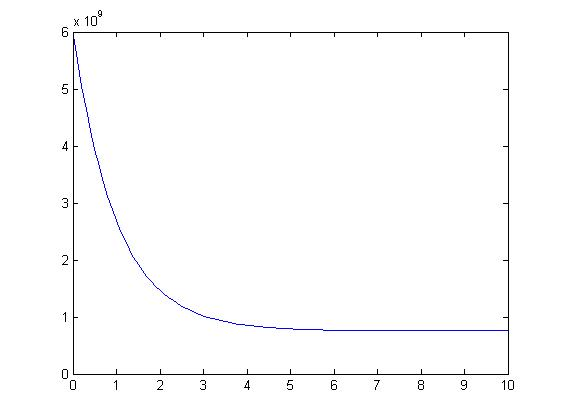
\includegraphics[scale=0.6]{./pic/duiliu.jpg}
%\caption{对流方程的图像,数据取自巨大芽孢杆菌对流方程}\label{pic:duiliu_nnn}
%\end{figure}
  \chapter{数值解}
对于大部分的偏微分方程模型问题来说,解得它们的解析解是比较困难的.在大部分的情况下,我们不能也没有必要求得它们的解析解.
因此,研究它们的数值解的求解方法是很有必要的.\par
在这一章中,我们同样从简单的方程开始解,建立数值解的求解方法的基本体系,然后我们再研究复杂模型的求解方法.
\section{常系数扩散方程}
考虑常系数扩散方程
\begin{equation}\label{eq:04_cxsks_o}
\begin{cases}
 \dfrac{\partial u}{\partial t}=a\dfrac{\partial^2 u}{\partial x^2} \\
 u(x,0)=g(x),\quad x\in\mathbb{R}
\end{cases}
\end{equation}
构成了初值问题,其向前差分格式为
\begin{gather}
 \dfrac{u_{j}^{n+1}-u_j^n}{\tau}-a\dfrac{u_{j+1}^n-2u_j^n+u_{j-1}^n}{h^2}=0,\label{eq:04_cxsks_xq}\\
 u_j^0 = g(x_j)
\end{gather}
其截断误差为$O(\tau+h^2)$.\par
考虑它的向后差分格式
\begin{equation}\label{eq:04_cxsks_xh}
 \dfrac{u_j^n-u_j^{n-1}}{\tau}-a\dfrac{u_{j+1}^n-2u_j^n+u_{j+1}^n}{h^2}=0
\end{equation}
其截断误差也是$O(\tau+h^2)$.
\subsection{加权隐式格式}
将式~\ref{eq:04_cxsks_xq}~改写为
\begin{equation}\label{eq:04_cxsks_xq_gx}
 \dfrac{u_j^n-u_j^{n-1}}{\tau}-a\dfrac{u_{j+1}^{n-1}-2u_{j}^{n-1}+u_{j-1}^{n-1}}{h^2}=0
\end{equation}
在式~\ref{eq:04_cxsks_xq}~乘以$\theta$,用$(1-\theta)$乘以~\ref{eq:04_cxsks_xq_gx},得到差分格式
\begin{equation}\label{eq:04_cxsks_js}
 \dfrac{u_j^n-u_j^{n-1}}{\tau}-a\left[\theta\dfrac{u_{j+1}^n-2u_j^n+u_{j-1}^n}{h^2}
 +(1-\theta)\dfrac{u_{j+1}^{n-1}-2u_j^{n-1}+u_{j-1}^{n-1}}{h^2}\right]=0
\end{equation}
其中,~$0\leq\theta\leq 1$,这种差分格式称为加权差分格式,将其改写为易于计算的格式
\begin{multline}
 -a\lambda\theta_{j+1}^n+(1+2a\lambda\theta)u_j^n-a\lambda\theta u_{j-1}^n = \\
 a\lambda(1-\theta)u_{j+1}^{n-1}+[1-2a\lambda(1-\theta)]u_j^{n-1}+a\lambda(1-\theta)u_{j-1}^{n-1}
\end{multline}
其中,$\lambda=\tau/h^2$,我们求差分格式~\ref{eq:04_cxsks_js}~的截断误差,设$u(x,t)$是方程~\ref{eq:04_cxsks_o}~的
充分光滑的解,在$(x_j,t_n)$处进行Taylor级数展开得
\begin{equation*}
E=a\left(\dfrac{1}{2}-\theta\right)\tau\left[\dfrac{\partial^3 u}{\partial x^2}{\partial t}\right]_j^n
+O(\tau^2+h^2)
\end{equation*}
当$\theta\not=1/2$时,其截断误差为$O(\tau+h^2)$.当$\theta=1/2$时,其截断误差为$O(\tau^2+h^2)$.\par
采用Fourier方法分析差分格式~\ref{eq:04_cxsks_js}~的稳定性,求得其增长因子为
\begin{equation}
 G(\tau,k)=\dfrac{1-4(1-\theta)a\lambda\sin^2\dfrac{kh}{2}}{1+4\theta a\lambda\sin^2\dfrac{kh}{2}}
\end{equation}
我们给出用于判断差分格式稳定性的\textbf{von Neumann}~定理,即
\begin{Theorem}[von Neumann定理]
差分格式
\begin{equation}
	u^{n+1}_j=C(x_j,\tau)u^n_j
\end{equation}
稳定的必要条件是当$\tau\leq\tau_0$,$n\tau\leq T$,对所有的k有
\begin{equation}
	\left|\lambda_j(G(\tau,k))\right| \leq 1+M\tau,\quad j=1,2,\cdots,p,
\end{equation}
其中$\left|\lambda_j(G(\tau,k))\right|$表示$G(\tau,k)$的特征值,$M$为常数。
\end{Theorem}\par
因此,要$|G(\tau,k)|\leq 1$,即
\begin{equation*}
 -1\leq\dfrac{1-4(1-\theta)a\lambda\sin^2\dfrac{kh}{2}}{1+4\theta a\lambda\sin^2\dfrac{kh}{2}}\leq 1
\end{equation*}
考虑左边的不等式,得
\begin{equation*}
4a\lambda(1-2\theta)\sin^2\dfrac{kh}{2}\leq2
\end{equation*}
因为$\sin^2\dfrac{kh}{2}\leq 1$,要求化为
\begin{equation}
 2a\lambda(1-2\theta)\leq 1.
\end{equation}
这是~\ref{eq:04_cxsks_js}~的稳定性要求.
\subsection{三层隐式格式}
考虑三层隐式差分格式,考虑
\begin{equation}\label{eq:04_cxsks_scys}
\dfrac{3}{2}\dfrac{u_j^{n+1}-u_j^n}{\tau}-\dfrac{1}{2}\dfrac{u_j^n-u_j^{n-1}}{\tau}
-a\dfrac{u_{j+1}^{n+1}-2u_{j}^{n+1}+u_{j-1}^{n+1}}{h^2}=0
\end{equation}
改写成便于计算的格式
\begin{equation}
 (3+4a\lambda)u_j^{n+1}-2a\lambda(u_{j+1}^{n+1}+u_{j-1}^{n+1})=4u_j^n-4u_j^{j-1}
\end{equation}
其中,~$\lambda=\tau/h^2$,易证差分格式~\ref{eq:04_cxsks_scys}~以二阶的精度逼近原微分方程.\par
将其化为等价的二层差分方程组
\begin{equation*}
\begin{cases}
(3+4a\lambda)u_j^{n+1}-2a\lambda(u_{j+1}^{n+1}+u_{j-1}^{n+1})=4u_j^n-v_j^n \\
v_j^{n+1}=u_j^n
\end{cases}
\end{equation*}
求得其增长矩阵为
\begin{equation*}
 G(\tau,k)=\begin{bmatrix}
  \dfrac{4}{3+8a\sin^2\dfrac{kh}{2}} & \dfrac{-1}{3+8a\sin^2\dfrac{kh}{2}} \\
                     1		     &			0		   \\
 \end{bmatrix}
\end{equation*}
其中,~$a=a\lambda$,$G$的特征方程为
\begin{equation*}
 \mu^2-\dfrac{4}{3+8\alpha\sin^2\dfrac{kh}{2}}\mu+\dfrac{1}{3+8\alpha\sin^2\dfrac{kh}{2}}=0
\end{equation*}
得$|\mu_i|\leq1(i=1,2)$.写出$\mu_i$的表达式
\begin{equation*}
\mu_{1,2}=\dfrac{2\pm\sqrt{1-8\alpha\sin^2\dfrac{kh}{2}}}{3+8\alpha\sin^2\dfrac{kh}{2}}.
\end{equation*}
若解为重根,显然有$|\mu_i|$,由此得出差分格式~\ref{eq:04_cxsks_scys}~是无条件稳定的.
\subsection{初边值问题}
我们考虑第一类边值问题,有
\begin{equation}
\begin{cases}
\dfrac{\partial u}{\partial t}-a\dfrac{\partial^2 u}{\partial x^2}=0,\quad 0<x<1,t>0 \\
u(x,0)=g(x),\quad 0\leq x\leq 1 \\
u(0,t)=\phi(t),\quad t\geq 0 \\
u(1,t)=\psi(t),\quad t\geq 0 
\end{cases}
\end{equation}
其计算区域为$x=[0,1]$,因此我们分开区间$0=x_0<x_1<\cdots<x_J=1$,第一边值问题的边界处理可取
\begin{equation}
\begin{cases}
u_0^n=\phi(t_n),\quad n\geq0 \\
u_J^n=\psi(t_n),\quad n\geq0
\end{cases}
\end{equation}\par
在初始线我们利用初始条件的离散
\begin{equation}
 u_j^0=g(x_j)=g_j
\end{equation}
得到边界点上的差分格式.\par
由于本研究不涉及第三类贬值条件,这一方面的差分处理方法就不叙述了.

\section{对流扩散方程}
考虑一个简单的对流扩散方程
\begin{equation}\label{equ:cf_dkfangc}
	\dfrac{\partial u}{\partial t}+a\dfrac{\partial u}{\partial x}=\nu\dfrac{\partial^2 u}{\partial x^2}
\end{equation}
其中a、$\nu$ 为常数,$\nu>0$,给定初值
\begin{equation}
	u(x,0)=g(x)
\end{equation}
构成了\textbf{对流扩散方程}的初值问题,在我们的模型中,它是一个对流占优的扩散问题。\par
\subsection{中心显式差分格式}
将方程~\ref{equ:cf_dkfangc}~差分,有
\begin{equation}\label{equ:cf_dkfangct}
	\dfrac{u^{n+1}_j-u^{n}_{j}}{\tau}+a\dfrac{u^{n}_{j+1}-u^n_{j-1}}{2h}=\nu\dfrac{u^n_{j+1}-2u^n_j+u^n_{j-1}}{h^2}
\end{equation}
其截断误差为$O(\tau+h^2)$。\par
下面来分析差分格式~\ref{equ:cf_dkfangct}~的稳定性,令
\begin{equation}
	\lambda = a\dfrac{\tau}{h},\quad\mu=\nu\dfrac{\tau}{h^2}
\end{equation}
则差分格式~\ref{equ:cf_dkfangct}~改写为
\begin{equation}\label{equ:cf_dkmmm}
u^{n+1}_j=u^n_j-\frac{1}{2}\lambda(u^n_{j+1}-u^n_{j-1})+\mu(u^n_{j+1}-2u^n_j+u^n_{j-1})
\end{equation}\par
式~\ref{equ:cf_dkmmm}~的增长因子为
\begin{equation}
	G(\tau,k)=1-2\mu(1-\cos kh)-i\lambda\sin kh
\end{equation}
模的平方为
\begin{equation}
\begin{aligned}
	|G(\tau,k)|^2 &= [1-2\mu(1-\cos kh)]^2+\lambda^2\sin^2 kh\\
				  &= 1-4\mu(1-\cos kh)+4\mu^2(1-\cos kh)^2+\lambda^2\sin^2 kh\\
				  &= 1-(1-\cos kh)[4\mu-4\mu^2(1-\cos kh)-\lambda^2(1+\cos kh)]
\end{aligned}				  
\end{equation}
差分格式稳定的充分条件为
\begin{equation}
4\mu-4\mu^2(1-\cos kh)-\lambda^2(1+\cos kh) \geq 0
\end{equation}
即
\begin{equation}
(2\lambda^2-8\mu^2)\dfrac{1-\cos kh}{2}+4\mu-2\lambda^2 \geq 0
\end{equation}
注意到$\dfrac{1}{2}(1-\cos kh)\in[0,1]$,上式应满足
\begin{equation}
(2\lambda^2-8\mu^2)+4\mu-2\lambda^2 \geq 0,\quad 4\mu-2\lambda^2 \geq 0
\end{equation}
由此得到差分格式~\ref{equ:cf_dkfangct}~的稳定性限制为
\begin{equation}
\tau \leq \dfrac{2\nu}{a^2}
\end{equation}
\begin{equation}
\nu\dfrac{\tau}{h^2}=\dfrac{1}{2}
\end{equation}\par
\subsection{迎风差分格式}
根据中心显式差分格式的稳定性要求可知,当$\nu/a^2$比较小时,时间步长是比较小的.我们在一阶空间偏导数的离散中采用单边差商,
令$a>0$,得到方程~\ref{equ:cf_dkfangc}~的迎风差分格式为
\begin{equation}\label{eq:cf_dkfangc_yf}
 \dfrac{u_j^{n+1}-u_j^n}{\tau}+a\dfrac{u_j^n-u_{j-1}^n}{h}=\mu\dfrac{u_{j+1}^n-2u_j^n+u_{j-1}^{n}}{h^2}
\end{equation}
容易看出,其截断误差为$O(\tau+h)$.\par
讨论其稳定性,将上式变为
\begin{equation}
 \dfrac{u_j^{n+1}-u_j^n}{\tau}+a\dfrac{u_{j+1}^n-u_{j-1}^n}{2h} = \left(\mu+\dfrac{ah}{2}\right)
 \dfrac{u_{j+1}^{n}-2u_j^n+u_{j-1}^n}{h^2}
\end{equation}
令$\bar{\mu}=\mu+\dfrac{ah}{2}$,可以得到式~\ref{eq:cf_dkfangc_yf}~的稳定性条件为
\begin{equation*}
\begin{split}
  \tau\leq&\dfrac{2}{a^2}\bar{\mu} \\[0.7em]
  \bar{\mu}\dfrac{\tau}{h^2}\leq&\dfrac{1}{2}
\end{split}
\end{equation*}
注意到,第一个稳定性条件等价于$\dfrac{\tau}{\dfrac{2\mu}{a^2}+\dfrac{h}{a}}\leq 1$,而
\begin{equation*}
\dfrac{\tau}{\dfrac{2\mu}{a^2}+\dfrac{h}{a}}=\dfrac{2\mu\dfrac{\tau}{h^2}\left(\dfrac{ah}{2\mu}\right)^2}{1+\dfrac{ah}{2\mu}}
\end{equation*}
利用不等式
\begin{equation*}
\dfrac{\left(\dfrac{ah}{2\mu}\right)^2}{1+\dfrac{ah}{2\mu}}\leq 1+\dfrac{ah}{2\mu}
\end{equation*}
这样得到
\begin{equation*}
\dfrac{\tau}{\dfrac{2\mu}{a^2}+\dfrac{h}{a}}\leq 2\mu\dfrac{\tau}{h^2}\left(1+\dfrac{ah}{2\mu}\right)
\end{equation*}
因此差分格式的稳定性条件为
\begin{equation}
 \left(\mu+\dfrac{ah}{2}\right)\dfrac{\tau}{h^2}\leq\dfrac{1}{2}
\end{equation}\par
迎风差分格式主要用于对流占优的扩散问题,采用中心差分格式不能很好地得出结果,采用迎风格式可以计算出问题的近似解.
\subsection{隐式差分格式}
考虑到隐性差分格式带来的诸多好处(如无条件稳定),给出迎风差分格式的隐式格式为
\begin{equation}\label{eq:04_yfcf_ys}
 \dfrac{u_j^{n+1}-u_j^n}{\tau}+a\dfrac{u_{j+1}^{n+1}-u_{j-1}^{n+1}}{2h}=\nu\sigma\dfrac{u_{j+1}^{n+1}
 -2u_j^{n+1}+u_{j-1}^{n+1}}{h^2}
\end{equation}
此格式是无条件稳定的.\par
现在考虑隐式差分格式的解法,将式~\ref{eq:04_yfcf_ys}~化为
\begin{equation*}
-\left(\dfrac{a}{2h}+\dfrac{\nu\sigma}{h^2}\right)u_{j-1}^{n+1}+\left(\dfrac{a}{2h}-\dfrac{\nu\sigma}{h^2}\right)u_{j+1}^{n+1}
+\left(\dfrac{1}{2}+\dfrac{2\sigma}{h^2}\right)u_j^{n+1}=\dfrac{1}{2}u_j^n
\end{equation*}
令
\begin{equation*}
\begin{aligned}
A_j &= -\dfrac{a}{2h}-\dfrac{\nu\sigma}{h^2} & \qquad & B_j = \dfrac{1}{2}+\dfrac{2\sigma}{h^2} \\[0.6em]
C_j &= \dfrac{a}{2h}-\dfrac{\nu\sigma}{h^2}  &  \qquad & D_j = \dfrac{1}{2}   \\
\end{aligned}
\end{equation*}
则方程可以写为
\begin{equation}\label{eq:04_yfcf_ys_b}
 A_j u_{j-1}^{n+1} + B_j u_j^{n+1} + C_j u_{j+1}^{n+1} = D_j
\end{equation}
其中,$j=1,2,\ldots,J-1$.我们令
\begin{equation}\label{eq:04_yfcf_ys_bj}
 u_0^{n+1}=0,\quad u_J^{n+1}=0
\end{equation}
为边界条件,方程~\ref{eq:04_yfcf_ys_b}~和方程~\ref{eq:04_yfcf_ys_bj}~构成系数为三对角矩阵的方程组,我们可以利用
追赶法求解这一方程组.\par
我们给出三对角矩阵存在Crout分解的充分条件,有
\begin{Theorem}[Crout分解的充分条件]
对于三对角矩阵
\begin{equation*}
A=\begin{bmatrix}
   b_1 & c_1 \\
   a_2 & b_2 & c_2 \\
       & a_3 & b_3    & c_3 \\
       &     & \ddots & \ddots  & \ddots            \\
       &     &        & a_{n-1} & b_{n-1} & c_{n-1} \\
       &     &        &         &   a_n   & b_n     \\
  \end{bmatrix}
\end{equation*}
存在Crout分解的充分条件为$a_i\not=0,(i=2,3,\ldots,n),c_1\not=0$,且
\begin{equation*}
\begin{split}
|b_1|&>|c_1|>0 \\
|b_i|&>|a_1|+|c_i|,(i=2,3,\ldots,n-1) \\
|b_n|&>|a_n|   \\
\end{split}
\end{equation*}
\end{Theorem}\par
方程~\ref{eq:04_yfcf_ys_b}~和方程~\ref{eq:04_yfcf_ys_bj}~的追赶法
求解充分条件为
\begin{equation}
\begin{cases}
|B_1|>|C_1|>0,\\
|B_j|\geq |A_j|+|C_j|,\quad A_j C_j\not=0,\quad j=2,\ldots,J-2,\\
|B_{J-1}|>|A_{J-1}| \\
\end{cases}
\end{equation}\par
利用矩阵的Crout分解解方程组,差分后得到的方程组可以写为
\begin{equation}~\label{eq:04_yfcf_jgmt}
\begin{bmatrix}
   B_1 & C_1 \\
   A_2 & B_2 & C_2 \\
       &  & \ddots    &  \\
       &     & A_j &  B_j    & C_j          \\
       &     &        &  & \ddots     \\
       &     &        &        &   A_{J-1}   & B_{J-1}     \\
\end{bmatrix}
\begin{bmatrix}
u_0^{n+1} \\
u_1^{n+1} \\
\vdots    \\
\vdots    \\
u_{J-2}^{n+1} \\
u_{J-1}^{n+1} \\
\end{bmatrix}
=
\begin{bmatrix}
D_0 \\
D_1\\
\vdots    \\
\vdots    \\
D_{J-2} \\
D_{J-1} \\
\end{bmatrix}
\end{equation}
对式~\ref{eq:04_yfcf_jgmt}~中的矩阵系数$A$进行Court分解,得
\begin{multline}
\begin{bmatrix}
   B_1 & C_1 \\
   A_2 & B_2 & C_2 \\
       &  & \ddots    &  \\
       &     & A_j &  B_j    & C_j          \\
       &     &        &  & \ddots     \\
       &     &        &        &   A_{J-1}   & B_{J-1}     \\
\end{bmatrix}=\\
\begin{bmatrix}
l_1 & \\
m_2 & l_2 \\
    & m_3 & l_3 \\
    &     & \ddots & \ddots & \\
    &     &        & m_{J-2} & l_{J-1} \\
    &	  &	   &	     &  m_{J-1} & l_{J-1} \\
\end{bmatrix}
\begin{bmatrix}
1 & u_0       \\
  &  1  & u_1 \\
  &     &   1  &  u_2 \\
  &     &      &   \ddots & \ddots \\
  &     &      &          &    1   & u_{J-1} \\
  &     &      &          &        &      1   \\
\end{bmatrix}
\end{multline}
其中,
\begin{equation}
\begin{cases}
m_i=a_i,\quad (i=2,3,\ldots,J-1) \\
l_1=b_1,u=c_1/l_1 \\
l_i=b_i-m_iu_{i-1},\quad (i=2,3,\ldots,J-1) \\
u_i=c_i/l_i,\quad (i=2,3,\ldots,J-2) 
\end{cases}
\end{equation}\par
利用
\begin{equation}
\begin{bmatrix}
l_1 & \\
m_2 & l_2 \\
    & m_3 & l_3 \\
    &     & \ddots & \ddots & \\
    &     &        & m_{J-2} & l_{J-1} \\
    &	  &	   &	     &  m_{J-1} & l_{J-1} \\
\end{bmatrix}
\begin{bmatrix}
y_0 \\
y_1 \\
y_2 \\
\vdots \\
y_{J-2} \\
y_{J-1} \\
\end{bmatrix}=
\begin{bmatrix}
 d_0 \\
 d_1 \\
 d_2 \\
 \vdots \\
 d_{J-2} \\
 d_{J-1} \\
\end{bmatrix}
\end{equation}
其中,
\begin{equation}
\begin{cases}
y_1=d_1/l_1 \\
y_i=(d_i-m_iy_{i-1})/l_i,\quad (i=2,3,\ldots,J-1)
\end{cases}
\end{equation}
解得$Y^{\mathrm{T}}$.\par
将$Y^{\mathrm{T}}$代入
\begin{equation}
\begin{bmatrix}
1 & u_0       \\
  &  1  & u_1 \\
  &     &   1  &  u_2 \\
  &     &      &   \ddots & \ddots \\
  &     &      &          &    1   & u_{J-1} \\
  &     &      &          &        &      1   \\
\end{bmatrix}
\begin{bmatrix}
x_0 \\
x_1 \\
x_2 \\
\vdots \\
x_{J-2} \\
x_{J-1} \\
\end{bmatrix}=
\begin{bmatrix}
y_0 \\
y_1 \\
y_2 \\
\vdots \\
y_{J-2} \\
y_{J-1} \\ 
\end{bmatrix}
\end{equation}
其中,
\begin{equation}
\begin{cases}
x_n=y_n \\
x_i=y_i-u_ix_{i+1},\quad (i=J-1,J-2,\ldots,1)
\end{cases}
\end{equation}
就解得了$X^{\mathrm{T}}$.
\section{多维方程}
多维方程是一维问题的推广,但是在求解的过程中会遇到诸多的问题.一维的差分格式直接拓展到多维上会导致稳定性条件变得严苛.若
采用隐式格式会无法使用追赶法从而导致求解困难.所以,在本节我们重点讨论多维方程差分格式的建立过程.
\subsection{二维扩散方程}
考虑二维上的扩散方程的初边值问题
\begin{equation}
\begin{cases}
\dfrac{\partial u}{\partial t}=a\left(\dfrac{\partial^2 u}{\partial x^2}+\dfrac{\partial^2 u}{\partial y^2}\right),& 0<x,y<1,\quad t>0, \\
u(x,y,0)=u_0(x,y),& 0<x,y<1 \\
u(0,y,t)=u(1,y,t)=u(x,0,t)=u(x,1,t)=0,& t>0
\end{cases}
\end{equation}
其中,~$a$为常数.\par
为了讨论差分格式,我们先将定义域
\begin{equation*}
D=\{(x,y,t)|0\leq x,y\leq 1,t\geq 0\}
\end{equation*}
划分网格
\begin{equation}
\begin{split}
D_h=\{(x_j,y_l,t_n)|x_j=jh,j=0,1,\ldots,J,Jh=1 \\
y_l=dh,l=0,1,\ldots,J;\quad t_n=n\tau,n\geq0\},
\nonumber
\end{split}
\end{equation}
其中,~$\tau$和$h$分别为时间步长和空间步长.我们考虑取$x$方向和$y$方向上的步长相等.引入记号
\begin{equation*}
\begin{split}
\delta_x^2 u_{jl}^n =& u_{j+1,l}^n-2u_{jl}^n+u_{j-1,l}^n, \\
\delta_y^2 u_{jl}^n =& u_{j,l+1}^n-2u_{jl}^n+u_{j,l-1}^n.
\end{split}
\end{equation*}



现在我们开始讨论在空间上建立和求解数学模型,根据运动控制方程,我们得到物质在空间上的分布为
\begin{equation}
 \dfrac{\partial u}{\partial t}=a\left(\dfrac{\partial^2 u}{\partial x^2}+\dfrac{\partial^2 u}{\partial y^2}
 +\dfrac{\partial^2 u}{\partial z^2}\right)-b\left(\dfrac{\partial u}{\partial x}+\dfrac{\partial u}{\partial y}
 +\dfrac{\partial u}{\partial z}\right)+cu+d
\end{equation}

  \chapter{数值模拟}
我们采用计算机来求解模型.为了简化编程,我们主要采用MATLAB矩阵实验室进行有限差分法的数值计算.\par
\section{扩散方程的模拟}
我们考虑这样简单的扩散方程,
\begin{equation}
\begin{cases}
\dfrac{\partial u}{\partial t}=\dfrac{\partial^ u}{\partial x^2}+2 & 0<x<1,t>0, \\
u(0,t)=u(1,t)=0,& t>1, \\
u(x,0)=sin(\pi x)+x(1-x).
\end{cases}
\end{equation}
我们采用六点差分格式来解这个方程,下面为用MATLAB编写的计算程序.
 \begin{lstlisting}[caption=六点差分格式,language=Matlab]
function [e]=six(dx,dt,t)
    m=1/dx;
    n=t/dt;
    u1=zeros(1,m+1);
    x=[1:m-1]*dx;
    u1([2:m])= sin(pi*x)+x.*(1 - x);
    r=dt/dx/dx;r2=2+2*r;r3=2-2*r;
    for i=1:m-1
	a(i,i)=r2;if i>1
	a(i-1,i)=-r;
	a(i,i-1)=-r;
	end;
    end
    for i=1:m-1
	b(i,i)=r3;
	if i>1
	    b(i-1,i)=r;
	    b(i,i-1)=r;
	end
    end
    u=zeros(n+1,m+1);
    u(n+1,:)=u1;
    for k=1:n
	b=b*(u(n+2-k,2:m))'+0.04;
	u(n+1-k,2:m)=inv(a)*b;
    end
    ut=u(1,:);
    x1=[0,x,1];
    plot(x1,ut,'*')
\end{lstlisting}
\begin{figure}[h]
 \centering
 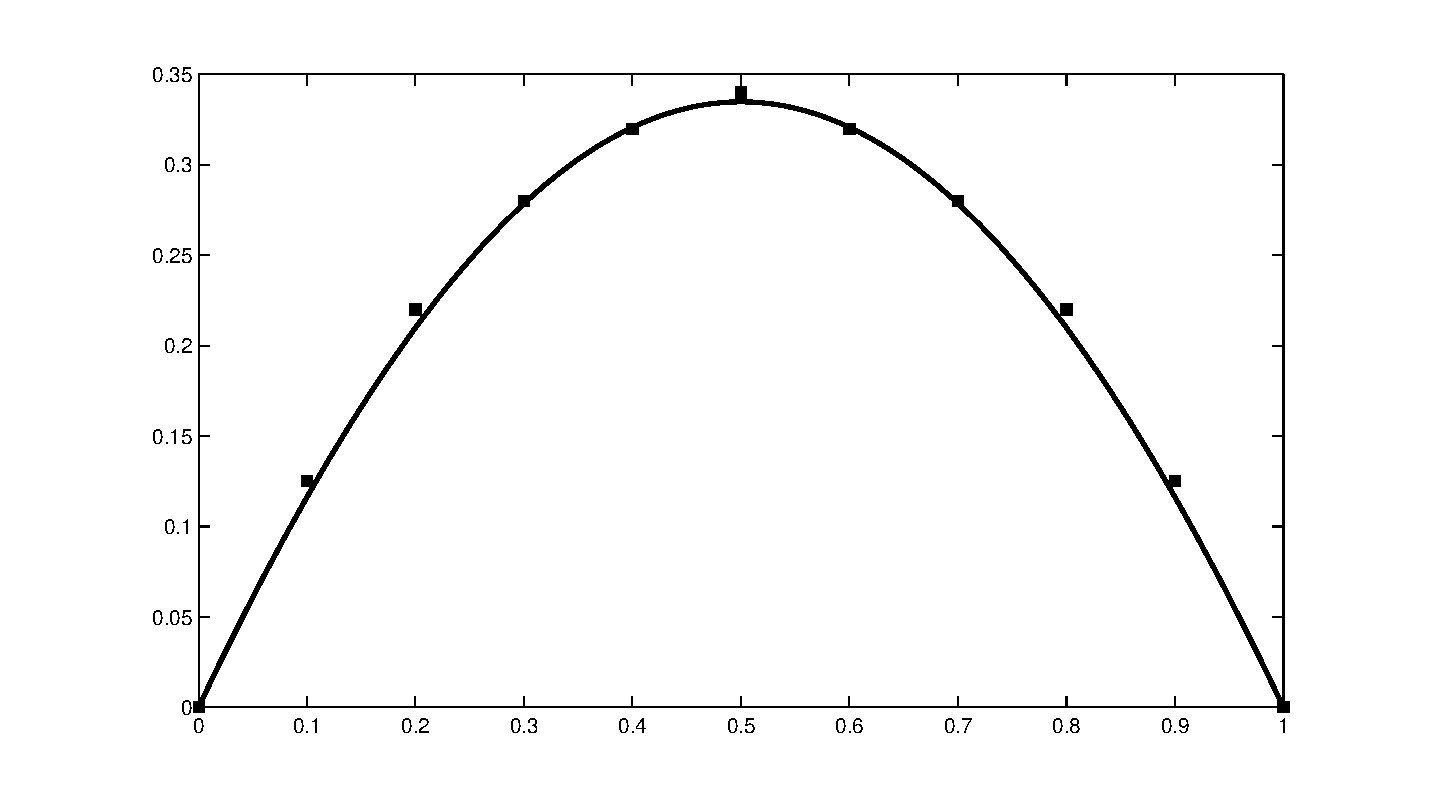
\includegraphics[scale=0.65]{./pic/6dcf.eps}
 \caption{扩散方程六点差分格式计算结果\label{fig:sm_ldcf}}
\end{figure}\par
仿真结果如图~\ref{fig:sm_ldcf}~所示,图中方块表示差分的数值结果,曲线表示解析结果.可以看到,虽然差分结果相对于解析解
是有误差的,但是误差不是很大.\newpage
\section{对流扩散方程的模拟}
考虑对流扩散方程
\begin{equation}\label{equ:cf_dkfangc}
	\dfrac{\partial u}{\partial t}+a\dfrac{\partial u}{\partial x}=\nu\dfrac{\partial^2 u}{\partial x^2}
\end{equation}
其中a、$\nu$ 为常数,$\nu>0$,给定初值
\begin{equation}
	u(x,0)=g(x)
\end{equation}
我们利用差分方法得到了一组差分方程,然后利用追赶法求解.
\begin{lstlisting}[caption=对流扩散方程差分求解,language=Matlab]
function C_k_1 = pencur3(Cin,u,A,B,D,E)
  M=2000;N=50;
  C_0=zeros(N+1,1);
  C_k_1=zeros(N+1,M);
  T=2500;L=40;
  t=T/M;
  h=L/N;
  a=B-2*A*u*h/D;
  AA=zeros(N+1);
  AA(1,1)=a;AA(1,2)=E+A;
  AA(N+1,N)=A+E;AA(N+1,N+1)=B;
  for i=2:N
      AA(i,i-1)=A;
      AA(i,i)=B;
      AA(i,i+1)=E;	
  end
  R=C_0;
  Rplus =-2*h*u*A/D*[1;zeros(N,1)];
  C_k_1(:,1)=C_0;
  for i=2:M
      R=C_k_1(:,i-1)+Rplus;
      C_k_1(:,i)=AA\R;
  end
  c=C_k_1;
  plot([1:M]',c(N+1,:));
  title('Curve');
  xlabel('t');
  ylabel('C/Cin');
end
\end{lstlisting}

\begin{figure}[h]
\centering
 \begin{floatrow}
 \ffigbox{\caption{对流扩散方程的差分计算结果1\label{fig:sm_dlfc1}}}{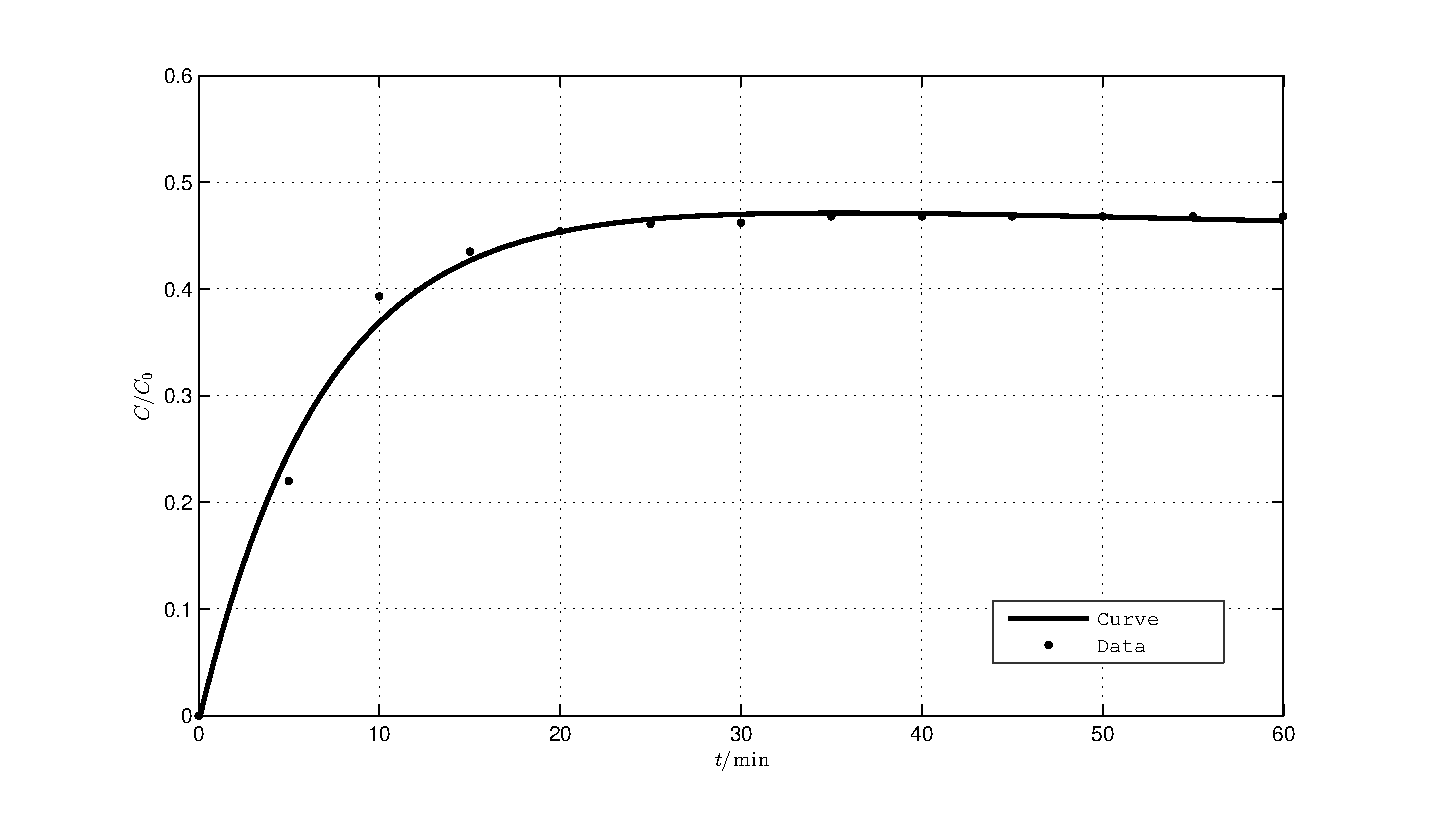
\includegraphics[scale=0.35]{./pic/dlfc.eps}}
 \ffigbox{\caption{对流扩散方程的差分计算结果2\label{fig:sm_dlfc2}}}{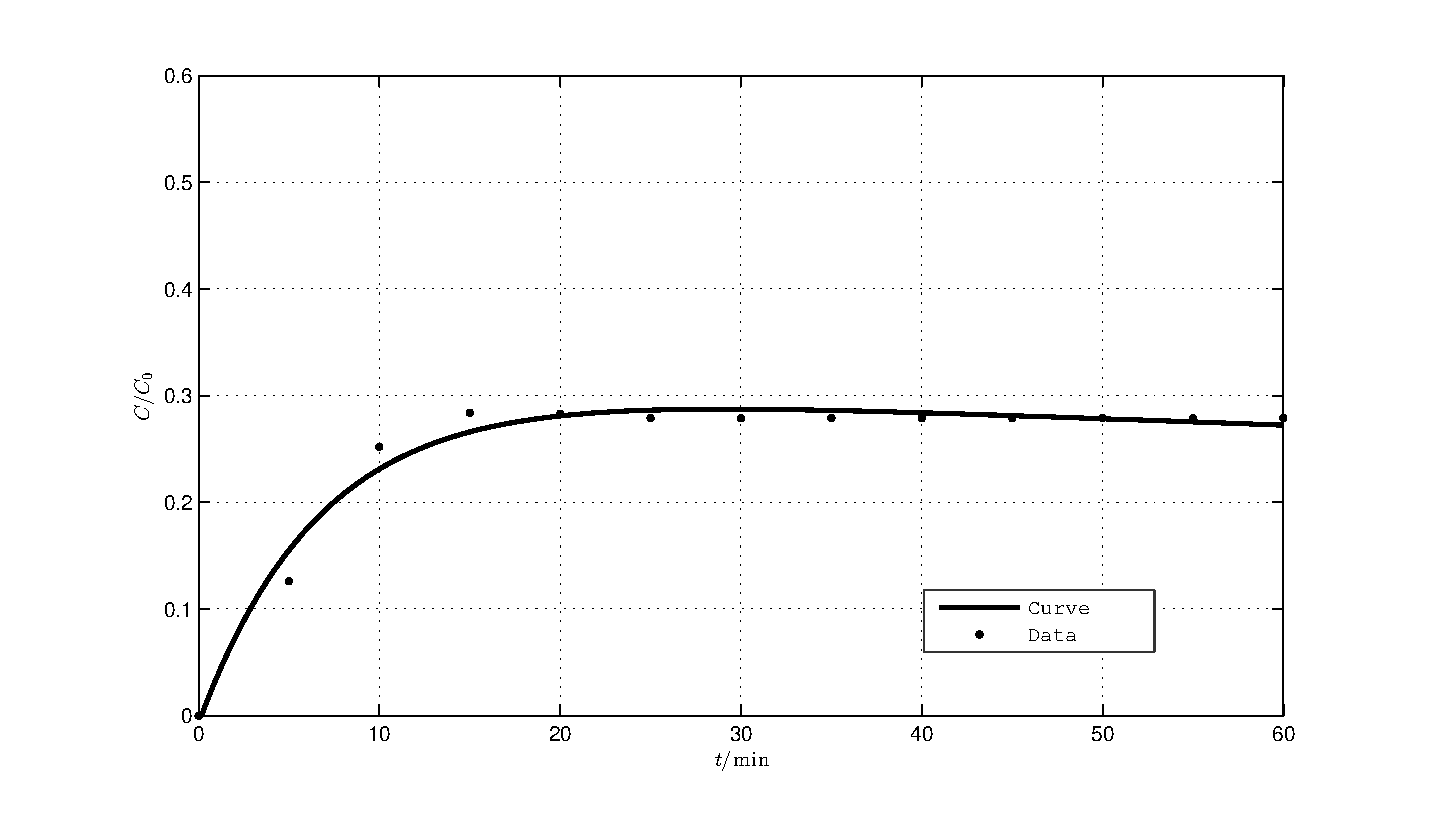
\includegraphics[scale=0.35]{./pic/dlfc2.eps}}
 \end{floatrow}
\end{figure}
% \begin{figure}[h]
%  \centering
%  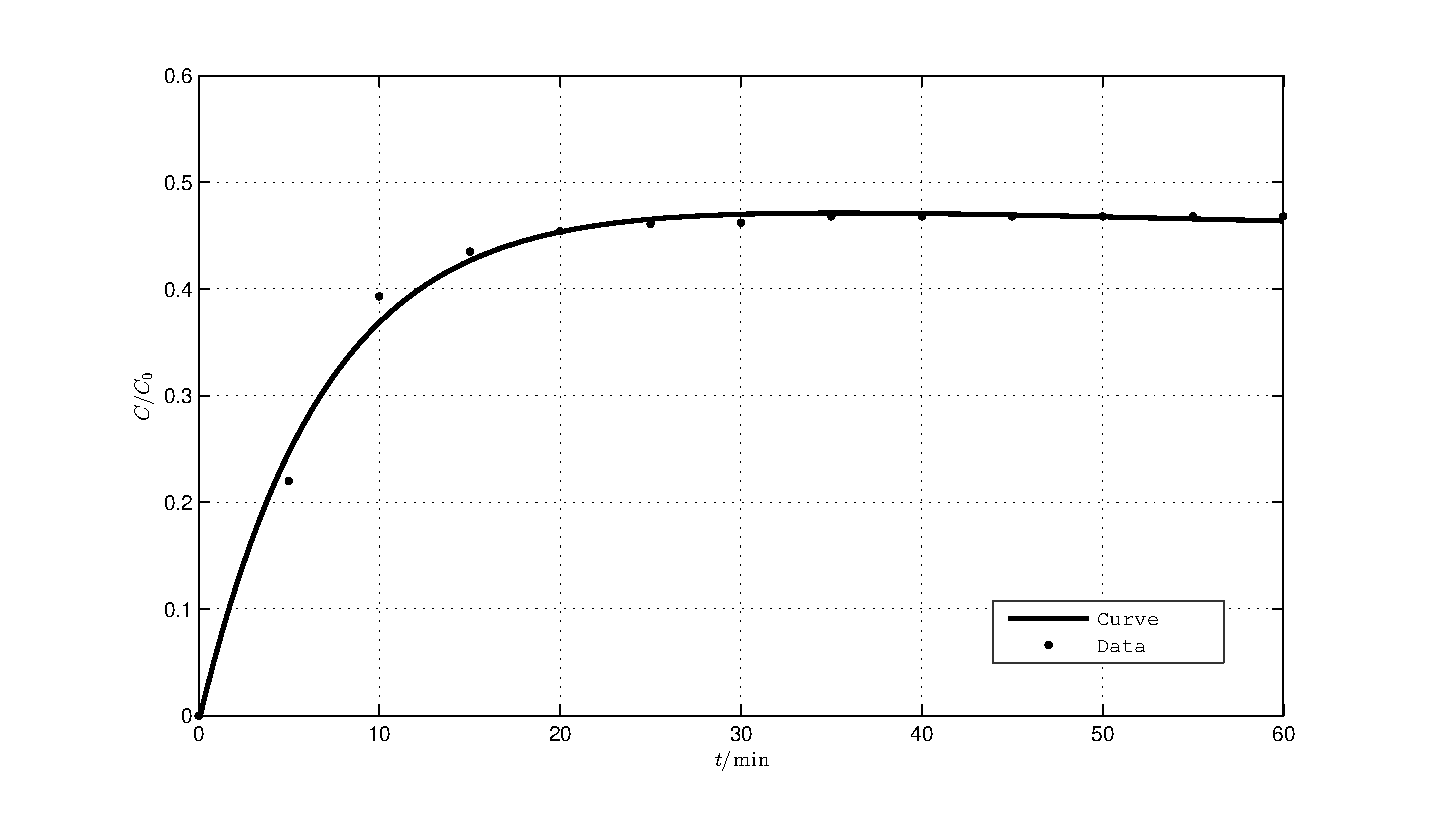
\includegraphics[scale=0.65]{./pic/dlfc.eps}
%  \caption{对流扩散方程(迎风格式)的差分计算结果1\label{fig:sm_dlfc}}
% \end{figure}\par
% \begin{figure}[h]
%  \centering
%  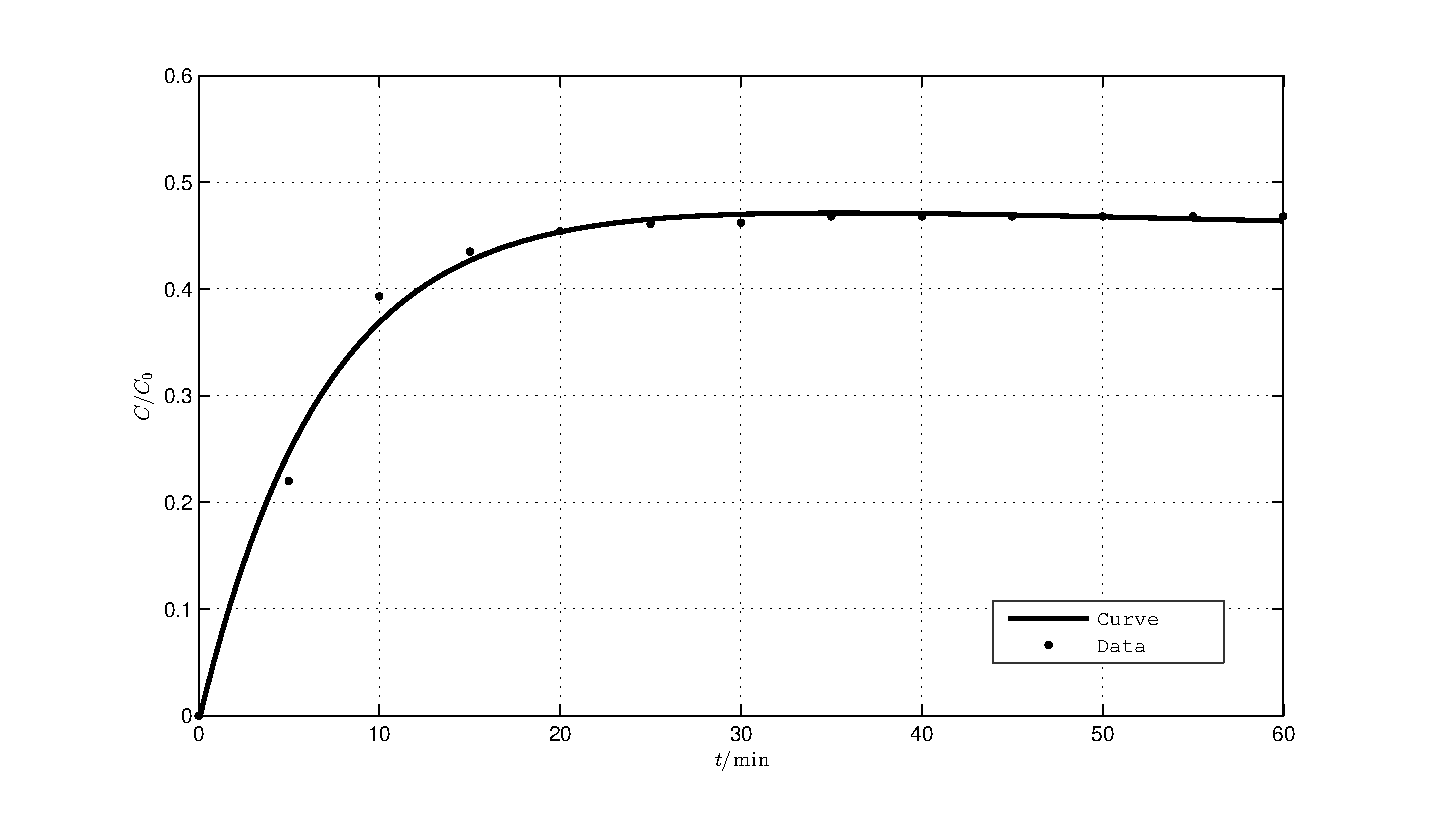
\includegraphics[scale=0.65]{./pic/dlfc.eps}
%  \caption{对流扩散方程(迎风格式)的差分计算结果2\label{fig:sm_dlfc2}}
% \end{figure}\par
图~\ref{fig:sm_dlfc1}~和图~\ref{fig:sm_dlfc2}~是对流扩散方程采用迎风格式的差分计算结果.其中,图线表示计算结果,方块是实验结果.我们看到,
模型在这个参数下可以较好地模拟实际的扩散情况.
\section{多维方程的模拟}
\begin{equation}\label{eq:sm_dw}
R_d\dfrac{\partial C}{\partial t}+v_i\dfrac{\partial C}{\partial x_i}=\dfrac{\partial}{\partial x_i}(D_{ij}\dfrac{\partial C}
{\partial x_j})-\mu C+\lambda,\quad (i,j=1,2,3)
\end{equation}
我们采用有限元法来求解这个方程,不考虑对流项,利用MATLAB工具箱,程序如下
\begin{lstlisting}[caption=有限元法,language=Matlab]
function pdemodel
[pde_fig,ax]=pdeinit;
pdetool('appl_cb',1);
set(ax,'DataAspectRatio',[1 0.0060000000000000001 1]);
set(ax,'PlotBoxAspectRatio',[250 166.66666666666666 50]);
set(ax,'XLim',[0 10]);
set(ax,'YLim',[-0.02 0.02]);
set(ax,'XTickMode','auto');
set(ax,'YTickMode','auto');

pderect([0 10 0.0050000000000000001 -0.0050000000000000001],'R1');
set(findobj(get(pde_fig,'Children'),'Tag','PDEEval'),'String','R1')

pdetool('changemode',0)
pdesetbd(4,...
'dir',...
1,...
'1',...
'6e8')
pdesetbd(3,...
'neu',...
1,...
'0',...
'0')
pdesetbd(2,...
'neu',...
1,...
'0',...
'0')
pdesetbd(1,...
'neu',...
1,...
'0',...
'0')

setappdata(pde_fig,'Hgrad',1.3);
setappdata(pde_fig,'refinemethod','regular');
setappdata(pde_fig,'jiggle',char('on','mean',''));
pdetool('initmesh')
pdetool('refine')
pdetool('refine')

pdeseteq(2,...
'3.66e-6',...
'1.035e-3',...
'7.819e5',...
'1.0',...
'0:10',...
'0.0',...
'0.0',...
'[0 100]')
setappdata(pde_fig,'currparam',...
['3.66e-6 ';...
'1.035e-3';...
'7.819e5 ';...
'1.0     '])

setappdata(pde_fig,'solveparam',...
str2mat('0','2016','10','pdeadworst',...
'0.5','longest','0','1E-4','','fixed','Inf'))

setappdata(pde_fig,'plotflags',[1 1 1 1 1 1 1 1 0 0 0 11 1 0 0 0 0 1]);
setappdata(pde_fig,'colstring','');
setappdata(pde_fig,'arrowstring','');
setappdata(pde_fig,'deformstring','');
setappdata(pde_fig,'heightstring','');
pdetool('solve')
\end{lstlisting}


  \chapter{结论与展望}

\backmatter
  \chapter{致谢}
首先要感谢我的导师周延老师.周老师在教学科研上严谨认真,学识渊博.在我完成毕业设计期间,尽心指导,亲力亲为,
不仅在理论上提出了诸多建议意见,在细节上也帮忙订正了许多错误,令我获益菲浅.不仅如此,周老师待人温和,对我非常关心,
在毕业期间对我个人前途和发展等诸多方面提出了很多建议,令我十分感动.非常感谢周老师对我的指导和帮助.\par
同时,感谢实验室的耿婧师姐.耿师姐在关于本课题的实验方面给了很多的指导,在历次检查过程中对报告的修改都给出了很多建议.\par
感谢理学院数学系黄晋阳教授在求解解析解过程中给予的帮助.\par
十分感谢我的本科生导师,同时也是我的研究生导师孙洪程高级工程师.\par
感谢辽阳市第一高级中学的张波老师和辽阳市新竹学校的乔立男校长、孙丽红老师和其他关心我成长的诸位老师.\par
感谢北京化工大学广播台的各位同事们,和你们共事四年,感到十分快乐和充实.我们有着共同的理想和生活态度,在这里
为了我们的理想挥洒青春和热血.有了你们,大学生活变得丰富多彩.祝你们在今后的生活中幸福快乐!\par

\end{document}